
%%%  یک نمونه پروپوزال کارشناسی ارشد، نسخه 0.4
%%%  وحید دامن‌افشان، دانشگاه تبریز،       http://www.damanafshan.ir
%%%   آپدیت شده در تیرماه ۹۱
%توضیحات مربوط به هر بسته یا دستور را می‌توانید در خط بالای آن ببینید.
%-----------------------------------
%%% شخصی‌سازی توسط نوید خزاعی (نخ) در اردیبهشت‌ماه ۹۳ - پروپوزال کارشناسی ارشد
\documentclass[12pt,a4paper]{article}
%در ورژن جدید زی‌پرشین برای تایپ متن‌های ریاضی، این سه بسته، حتماً باید فراخوانی شود
\usepackage{amsthm,amssymb,amsmath}

%دستوری برای وارد کردن واژه‌نامه انگلیسی به فارسی
\newcommand\persiangloss[2]{#1\dotfill\lr{#2}\\}
%%% ------- اضافه شده توسط نخ ------

\numberwithin{equation}{section}
\numberwithin{figure}{section}


%Make section number before figure number.
\renewcommand{\thefigure}{\arabic{figure}.\thesection}
\renewcommand{\theequation}{\arabic{equation}.\thesection}
\renewcommand\thetable{\arabic{table}.\thesection}

\usepackage{wrapfig}
\usepackage{mathabx}
%%% دستوری برای پنهان کردن چیزی از فهرست

\newcommand{\nocontentsline}[3]{}
\newcommand{\tocless}[2]{\bgroup\let\addcontentsline=\nocontentsline#1{#2}\egroup}
\usepackage[bottom]{footmisc}
\usepackage{indentfirst}
%\usepackage[english]{babel}
%\usepackage{caption}
%\captionsetup[figure]{name=شکل}

%\captionsetup[contentsname]{name=فهرست}
%\renewcommand{\contentsname}{فهرست مطالب}

% ------ پایان تغییرات نخ
%بسته‌ای برای تنطیم حاشیه‌های بالا، پایین، چپ و راست صفحه
%\usepackage[top=50mm, bottom=50mm, left=50mm, right=50mm]{geometry}
%بسته‌ای برای نمایش تصاویر قرار داده شده در متن
\usepackage{graphicx}
\usepackage{subcaption}
% بسته‌ و دستوراتی برای ایجاد لینک‌های رنگی با امکان جهش
\usepackage[pagebackref=false,colorlinks,linkcolor=blue,citecolor=magenta]{hyperref}
% چنانچه قصد پرینت گرفتن نوشته خود را دارید، خط بالا را غیرفعال و  از دستور زیر استفاده کنید چون در صورت استفاده از دستور زیر‌‌، 
% لینک‌ها به رنگ سیاه ظاهر خواهند شد و برای پرینت گرفتن، مناسب‌تر خواهد بود.
%\usepackage[pagebackref=false]{hyperref}
%بسته‌ای برای ظاهر شدن «مراجع»  در فهرست مطالب
\usepackage{tocbibind}
%فراخوانی بسته زی‌پرشین و دستورات مربوط به نوع فونت‌ها
\usepackage{xepersian}
\settextfont[Scale=1.1]{B Nazanin}
\DefaultMathsDigits
\usepackage{zref-perpage}
\zmakeperpage{footnote}
% وارد کردن دستور بالا الزامی نیست؛ چون در صورت وارد نکردن آن، فونت پیش‌فرض به صورت خودکار، فراخوانی می‌شود.
% چنانچه می‌خواهید که اعداد داخل فرمول‌ها، فارسی باشد، دستور زیر را فعال کنید
%\setdigitfont{Yas}
%%%%%%%%%%%%%%%%%%%%%%%%%%%%%%%%%%%%%%%%%%%%%%%%%%%
% تعریف قلم‌های فارسی و انگلیسی برای استفاده در بعضی از قسمت‌های متن
\defpersianfont\titr[Scale=1]{B Titr}
\defpersianfont\nastaliq[Scale=1.5]{IranNastaliq}
\defpersianfont\traffic[Scale=1]{B Traffic}
\defpersianfont\yekan[Scale=1]{B Yekan}
%اگر فونت‌های بالا را ندارید، دو خط بالا را غیر فعال و دو خط زیر را فعال کنید
%\defpersianfont\traffic[Scale=1]{XB Roya}
%\defpersianfont\yekan[Scale=1]{XB Kayhan}
%%%%%%%%%%%%%%%%%%%%%%%%%%%%%%%%%%%%%%%%%%%%%%%%%%%
% تعریف و نحوه ظاهر شدن قضایا، لم‌ها، تعریف‌ها و ...
\theoremstyle{definition}
\newtheorem{definition}{تعریف}[section]
\theoremstyle{theorem}
\newtheorem{theorem}[definition]{قضیه}
\newtheorem{lemma}[definition]{لم}
\newtheorem{proposition}[definition]{گزاره}
\newtheorem{corollary}[definition]{نتیجه}
\newtheorem{remark}[definition]{ملاحظه}
\theoremstyle{definition}
\newtheorem{example}[definition]{مثال}
%%%%%%%%%%%%%%%%%%%%%%%%%%%%%%%%%%%%%%%%%%%%%%%%%%%
\begin{document}
% دستوری جهت حذف کردن شماره صفحه و سربرگ، در صورت وجود (فقط در صفحه جاری)
\thispagestyle{empty}
\vspace*{-28mm}
% نحوه درج کردن لوگوی دانشگاه
\centerline{
\includegraphics[height=5cm]{logo.png}}
\begin{center}
%دستوری برای کم کردن فاصله بین لوگو و خط پایین آن
\vspace{-6mm}

گروه مستقل مهندسی رباتیک
%دستوری برای تعیین فاصله بین دو خط
\\[1.5cm]

{\large
\textbf { 
گزارش مطالعاتی درس بینایی ربات
}
\\[1.2cm]
عنوان:
\\[.4cm]
}
%دستوری برای تعیین فاصله بین خطوط (نه دو خط) و تا وقتی که مقدار آن تغییر نکند، فاصله بین خطوط، همین مقدار است.
\baselineskip=1cm
{\Large \titr
تشخیص بیضی
\\[1cm]
}

{\Large \titr
\lr{ 
\textbf{Ellipse Detection
}
\\[.6cm]
}
\vspace{-9mm}
}

{\large
استاد درس:
}
\\[.3cm]
\textbf{\large {\nastaliq دکتر رضا صفابخش}}
\\[.5cm]

{\large
 پژوهشگر:
}
\\[.3cm]
\textbf{\large {\nastaliq نوید خزاعی}}
\\[.5cm]
{\large
تیر ۱۳۹۳
}
\end{center}
%دستوری برای رفتن به صفحه جدید
\newpage
\baselineskip=1cm

\baselineskip=.75cm
\newpage 
\pagenumbering{Alph}
\tocless {\section*}{چکیده}

برای تشخیص بیضی، روش‌های معمول یا مبتنی بر تبدیل هاف هستند، یا بر مبنای ویژگی‌های هندسی بیضی و ابتکاری هستند. در این گزارش برخی روش‌های موجود را برشمردیم و در برخی موارد تحلیلی از چگونگی عملکرد و مشکلات و بهبودها ارایه کردیم. سه مورد از روش‌های مبتنی بر تبدیل هاف، و یک مورد از روش‌های ابتکاری را نیز به شکل جزیی‌تر بررسی کردیم و اشاره‌ای نیز به مقایسه‌های موجود در مقالات نموده‌ایم. 

\newpage
\tocless\tableofcontents
\newpage 
\pagenumbering{arabic}
\section{مقدمه}
تشخیص اشیا و اشکال هندسی، همواره یکی از چالش‌برانگیزترین موضوعات در بینایی ماشین بوده‌است. در این میان، دایره و بیضی از اهمیت بیشتری برخوردارند. بیضی حالت عام‌تری از دایره است چرا که دایره همان بیضی است که نیم‌قطر کوچک و نیم‌قطر بزرگ آن مساوی است. در تصاویر واقعی، افکنش‌های دایره‌های موجود ممکن است به شکل بیضی در تصویر ظاهر شوند. همچنین در بسیاری از موارد دایره‌های ایده‌آل نداریم و کشیدگی‌ها و ناهمواری‌ها سبب می‌شود تا شکل‌ها بیشتر شبیه بیضی باشند. از این رو، تشخیص بیضی‌ها در پردازش تصاویر واقعی می‌تواند بسیار موثر باشد و درک ما از تصویر را افزایش بدهد. همچنین می‌توان اشکال را ویژگی‌هایی برای توصیف شکل دانست و با توجه به کاربرد مساله، هر تصویر را با اشکال موجود توصیف کرد. با این وصف، حجم مجموعه‌ی داده‌ها کاهش داده‌می‌شود، بنابراین می‌توان از این مجموعه‌ی برای حل مساله‌ی مورد نظر، و یا به عنوان ورودی برای پردازش‌های آتی، استفاده نمود. 

در ریاضیات، بیضی یک خم مسطح (خم محصور در صفحه‌ی اقلیدسی)، از خانواده‌ی مخروطی‌ها\LTRfootnote{ Conics} و یک مقطع مخروطی محدود است. مقطع مخروطی حاصل از قطع دادن یک صفحه با یک مخروط دایره‌ای است. خم‌های دیگری نیز از قطع کردن مخروط به‌دست می‌آیند که نامحدود هستند و سهمی و هذلولی نام دارند \cite{Wiki}. همان‌گونه که اشاره شد، بیضی از دایره عمومی‌تر است و در ریاضیات نیز، معیاری برای سنجش انحراف بیضی از دایره‌ی معادل وجود دارد که به آن گریز از مرکز\LTRfootnote{ Eccentricity} می‌گویند. این ارتباط، خود می‌تواند اطلاعاتی در مورد اندازه و جهت به‌دست دهد که در کاربردهای زیادی مورد استفاده قرار می‌گیرد. محققان کاوش‌های زیادی برروی ویژگی‌های بیضی انجام داده‌اند که از جمله‌ی آن‌ها می‌توان به استفاده از طبیعت متقارن کانون‌ها\LTRfootnote{ Foci} برای پارامتری کردن بیضی اشاره نمود \cite{param}. همچنین از ارتباط توام قطرها بین وترهای موازی برای پیش‌بینی مرکز بیضی استفاده شده‌است \cite{diam}. 

تشخیص دقیق بیضی در کاربردهای بی‌درنگ بسیار مهم است، چرا که دقت تشخیص می‌تواند به‌خاطر رسیدن به پاسخ‌گویی با نرخ بالاتر، کاهش یابد. از جمله کاربردهای تشخیص بیضی می‌توان به موارد زیر اشاره کرد: 

\begin{itemize}
\renewcommand{\labelitemi}{$\bullet$}
\item 
\textbf{نظارت و دیده‌بانی: } 
دنبال کردن چشم، لب‌‌خوانی، و تشخیص چهره به شدت بر مبنای تشخیص بیضی انجام می‌شود. همچنین دنبال کردن اعضای انسان می‌تواند با دنبال کردن چندین بیضی انجام شود که برای تشخیص برخی اعمال مانند افتادن، کاربرد دارد. استفاده از بیضی در این مورد بهتر از کادر دور شخص است چرا که بیضی جهت و شکل شخص را نیز حفظ می‌کند.

\item
\textbf{کشاورزی: }
محاسبه‌ی اندازه و مقایسه‌ی محصولات، می‌تواند در مرتب‌سازی و چیدن خودکار مورد استفاده قرارگیرد. 

\item 
\textbf{صنعت: }
گریز از مرکز سیم‌پیچ‌های فولادی می‌تواند معیاری برای کنترل کیفیت باشد.

\item 
\textbf{زیست‌پزشکی: }
سلول‌ها را می‌توان با تشخیص بیضی، تقطیع کرد و با کمک بیضی‌های چندگانه می‌توان مدل سه‌بعدی از سلول را ساخت. به عنوان نمونه‌ای دیگر، می‌توان حجم یک پروستات بیضی‌شکل را با لایه‌هایی از بیضی‌ها تخمین زد.

\item 
\textbf{اقیانوس‌شناسی: }
گرداب‌های بیضی‌شکل بسیاری در نقشه‌های دمای سطح\LTRfootnote{ Surface TemperaTure maps (STT)} اتفاق می‌افتد.

\item 
\textbf{نقشه‌برداری فضایی: }
کمان‌های بیضی‌گون در تصاویر ماهواره‌ای از کانتورهای طبیعی موجود در سیارات و نیز سازه‌های دست بشر، به چشم می‌خورند.

\item 
\textbf{کاوش‌های فضایی:‌ } 
هاله‌های نوری خورشید شکل‌های بیضی‌گون دارند و اطلاعات به‌دست آمده از اندازه و جهت آن‌ها در موقعیت‌یابی مفید است.


\item 
\textbf{رباتیک: }
در مسایل بسیاری از جمله تشخیص تابلوهای راهنمایی و رانندگی در خودروهای هوشمند، تشخیص توپ در زمین فوتبال و غیره کاربرد دارد.

در این گزارش، در بخش دوم به بررسی روش‌های موجود برای تشخیص بیضی خواهیم‌پرداخت و در بخش‌های سوم تا پنجم، سه نمونه را با توجه به اهمیت کاربرد و درک الگوریتم آن‌ها به صورت جزیی‌تر بررسی خواهیم‌کرد.

\end{itemize}

\newpage

\section{الگوریتم‌های تشخیص و کارهای مرتبط}

تمامی الگوریتم‌های تشخیص بیضی، بر مبنای ویژگی‌های هندسی یکتای بیضی کار می‌کنند. برای سادگی، برخی ویژگی‌ها در شکل \ref{fig:ellipse} آورده شده‌است. 

\begin{figure}[h]
\centering
\frame{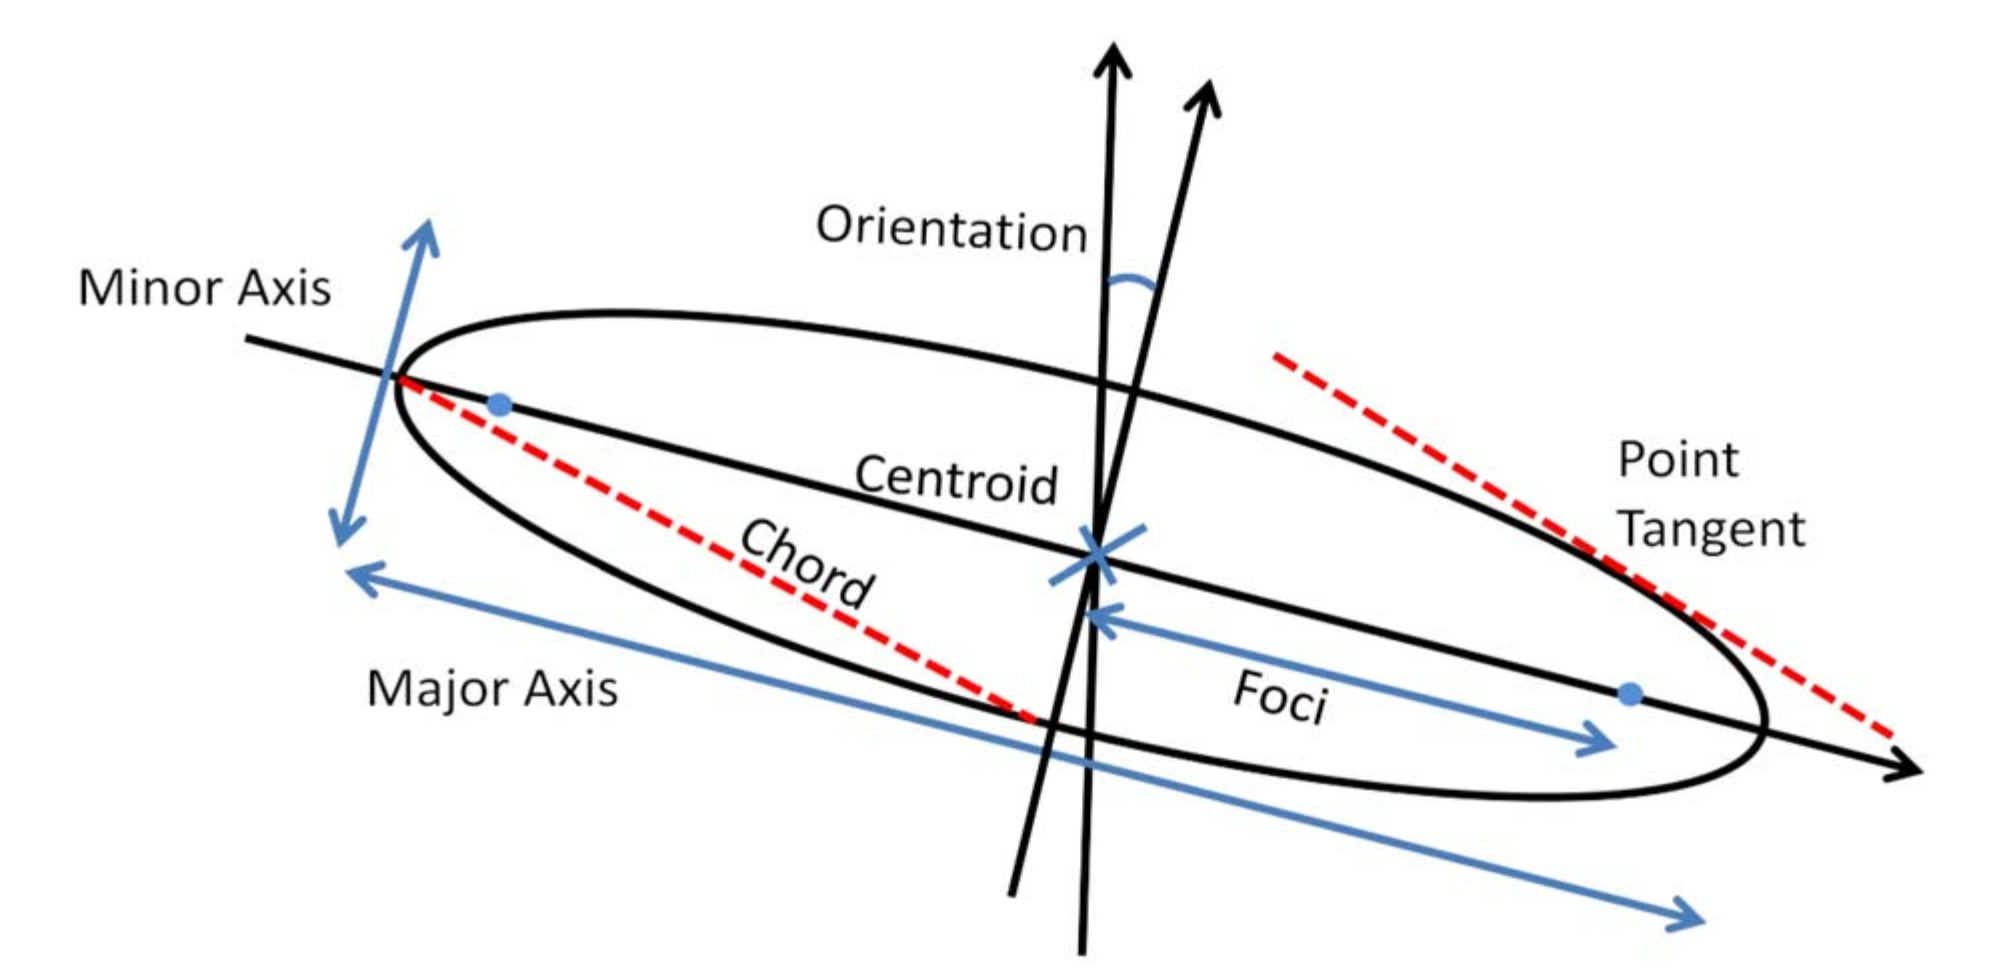
\includegraphics[height=5.5cm]{ellipse.png}}
\caption{پارامترهای بیضی (آبی) و ویژگی‌های هندسی بیضی (قرمز)\cite{survey}. }
\label{fig:ellipse}
\end{figure}

پارامترهای بیضی عبارت‌اند از مرکز (مرکز ثقل\LTRfootnote{ Centroid})، نیم‌قطر کوچک\LTRfootnote{ Minor Axis}، نیم‌قطر بزرگ\LTRfootnote{ Major Axis}، جهت و کانون‌ها\LTRfootnote{ Foci}. 

ویژگی‌های هندسی شامل وتر\LTRfootnote{ Chord} و تانژانت نقطه\LTRfootnote{ Point Tangent} می‌باشد که به ترتیب حاصل از اتصال دو نقطه‌ روی محیط بیضی و حاصل از قطع دادن مماس در یک نقطه با امتداد نیم‌قطر بزرگ می‌باشند. 

در ادبیات موضوع، روش‌های برازش بیضی به داده‌ها نیز از روش‌های تشخیص بیضی شمرده شده‌است. با این حال در گزارش پیش رو از بررسی این روش‌ها خودداری کردیم چرا که نسبت به روش‌های دیگر،‌ کمتر از تکنیک‌های بینایی ماشین و پردازش تصویر استفاده می‌کنند و مساله‌ی برازش بیضی به داده‌ها، بسیار عام‌تر از تشخیص بیضی در تصاویر است.

به این ترتیب، می‌توان روش‌های باقی‌مانده را به دو دسته‌ی کلی تقسیم کرد: روش‌های مبتنی بر رای‌گیری یا خوشه‌بندی، و روش‌های ابتکاری یا ترکیبی. در ادامه به بررسی کارهای انجام‌شده در این زمینه خواهیم پرداخت و پس از آن، دو نمونه‌ی پرکاربرد از دسته‌ی اول و یک نمونه‌ی برگزیده از دسته‌ی دوم را معرفی خواهیم کرد. 

\subsection{روش‌های مبتنی بر رای‌گیری یا خوشه‌بندی}


روش‌های خوشه‌بندی فازی همانند \cite{fuzzy}، مقاومت را فدای تشخیص سریع می‌کردند و قبل از به وجود آمدن روش مبتنی بر رای‌گیریِ «تبدیلِ هاف»\LTRfootnote{ Hough Transform (HT)} استفاده می‌شدند. روش هاف یکی از محبوب‌ترین و پرکاربردترین الگوریتم‌ها در بینایی ماشین است که در \cite{hough} برای تشخیص ویژگی‌های هندسی مانند خط و مخروطی‌ها معرفی شد که در درس بینایی ماشین به طور مفصل با آن آشنا شدیم. همچنین دیدیم که برای ورودی این تبدیل، به کاربردن یک عملگر لبه‌یابی مناسب، حیاتی است. در دهه‌های اخیر، تبدیل هاف بهبودهای زیادی پیدا کرده‌است تا محدودیت‌ها و کاربردهای بسیاری را از جمله تشخیص بیضی و کمان‌های بیضی‌گون پوشش دهد. 

برخی از روش‌های هاف، از جمله خود تبدیل استاندارد هاف و بهبودهای بسیاری از آن، مانند هاف احتمالاتی\LTRfootnote{ Probabilistic HT}، هاف تصاعدی\LTRfootnote{ Progressive PT}، هاف ترکیبیاتی\LTRfootnote{ Combinatorial HT} و هاف تقارن هندسی\LTRfootnote{ Geometric Symmetry HT}، که برای تشخیص خط بسیار موثر هستند، برای تشخیص چندین بیضی موثر نیستند. چرا که برای توصیف فضای پارامتری بیضی، نیاز به ۵ متغیر (۵ پارامتر بیضی) داریم، حال آن‌که برای فضای پارامتری خط تنها دو متغیر داشتیم. بدیهی است که سربار محاسباتی و نیاز به منابع پردازشی با افزایش پارامترها به صورت نمایی رشد می‌کند. جست‌وجو به دنبال قله‌ی موجود در چنین آرایه‌ی انباره‌ای\LTRfootnote{ Accumulator array} خود به تنهایی زمان‌بر است. با این حال، مقاومت روش‌ هاف در برابر پوشیدگی\LTRfootnote{ Occlusion} سبب شده‌است محققان به بهبود این روش برای تشخیص بیضی ادامه‌دهند. 

روش‌های هاف موجود برای تشخیص چندین بیضی به ترتیب زمان پیدایش عبارت‌اند از: 
هاف عمومی\LTRfootnote{ Generalized HT (GHT)}\cite{GHT}، 
هاف خط مستقیم\LTRfootnote{ Straight Line HT (SLHT)}\cite{SLHT}، 
تبدیل هاف سریع بیضی\LTRfootnote{ Fast Ellipse Hough Transform (FEHT)}\cite{FEHT} 
و هاف تصادفی‌\LTRfootnote{ Randomized HT (RHT)}\cite{RHT}.

تبدیل هاف را می‌توان با استفاده از جهت‌های لبه‌ها و با ساختن جدول‌های توصیف‌گر شکل\LTRfootnote{ R-Table} که در \cite{GHT} آورده شده‌است، برای هر شکلی عمومی کرد. در اصل روش هاف عمومی، تلاش می‌کند با شکستن شکل به قطعه‌های کوچک‌تر، فضای پارامتر را کم کند و پیچیدگی را کاهش دهد.

در \cite{SLHT} روشی برای تشخیص بیضی با روش هاف ارایه شده‌است که نیازی به آرایه‌ی انباره ندارد. این روش مرکز بیضی‌ها را با توجه به اثر بیضی در \lr{SLHT} و اصول نصف کردن قطر\LTRfootnote{ Diameter Bisection} پیدا می‌کند. پارامتری در فضای تبدیل هاف معرفی شده‌است که به کمک آن می‌توان با استفاده از یک الگوریتم تشخیصِ خوشه‌ی ساده، بیضی‌ها را پیدا کرد و نیازی به جست‌وجوی قله‌ها در آرایه‌ی انباره نیست. پیچیدگی زمانی تابع اصلی در این روش 
\( O(n^2) \)
است. 

\lr{FEHT}
 با روش سرکشی معمول در روش هاف تفاوت دارد، چرا که اساس آن یک روش تکراری تمرکزکردن\LTRfootnote{ Focusing}
است\cite{FEHT}. این روش برای وقتی که بیضی‌هایی با اندازه‌های متفاوت به دفعات زیاد در تصویر ظاهر می‌شوند مفید است و می‌تواند آن‌ها را از هم تفکیک کند. در این گزارش به بررسی دقیق‌تر این روش در بخش سوم خواهیم پرداخت. 

\lr{RHT}
بر مبنای تخمین تانژانت‌های محلی است تا با این کار، مساله‌ی غیرخطی را به یک مساله‌ی خطی کاهش دهد. در این روش، انبار کردن نقاط فضای پارامتری با انتخاب تصادفی چندتایی‌هایی از پیکسل‌ها و محاسبه‌ی پارامترهای شکلی که از این پیکسل‌ها عبور می‌کند، انجام می‌شود\cite{RHT}. در بخش چهارم از این گزارش به بررسی دقیق‌تر این روش نیز خواهیم پرداخت.

در \cite{ellipticalHT} تبدیل هاف با یک هرم تصویر ترکیب شده‌است و یک تشخیص بیضی مقاوم به دست آمده‌است. تصویر با کم‌ترین کیفیت، نقطه‌ی شروع در این روش است و با افزایش کیفیت تصویر، بیضی‌های کاندید توسط به روز رسانی یک هافِ چندگذره\LTRfootnote{ Multi pass HT} محاسبه می‌شوند، به این ترتیب که نقاط حاصل از کیفیت جدید، نقاط حاصل از تصویر قبلی در فضای پارامتری را به‌روزرسانی می‌کنند. برای درک بهتر به شکل \ref{fig:elliptic} مراجعه کنید. پیچیدگی زمانی تابع اصلی در این روش 
\( O(n^{5/2}) \)
است. 
\begin{figure}[h]
\centering
\frame{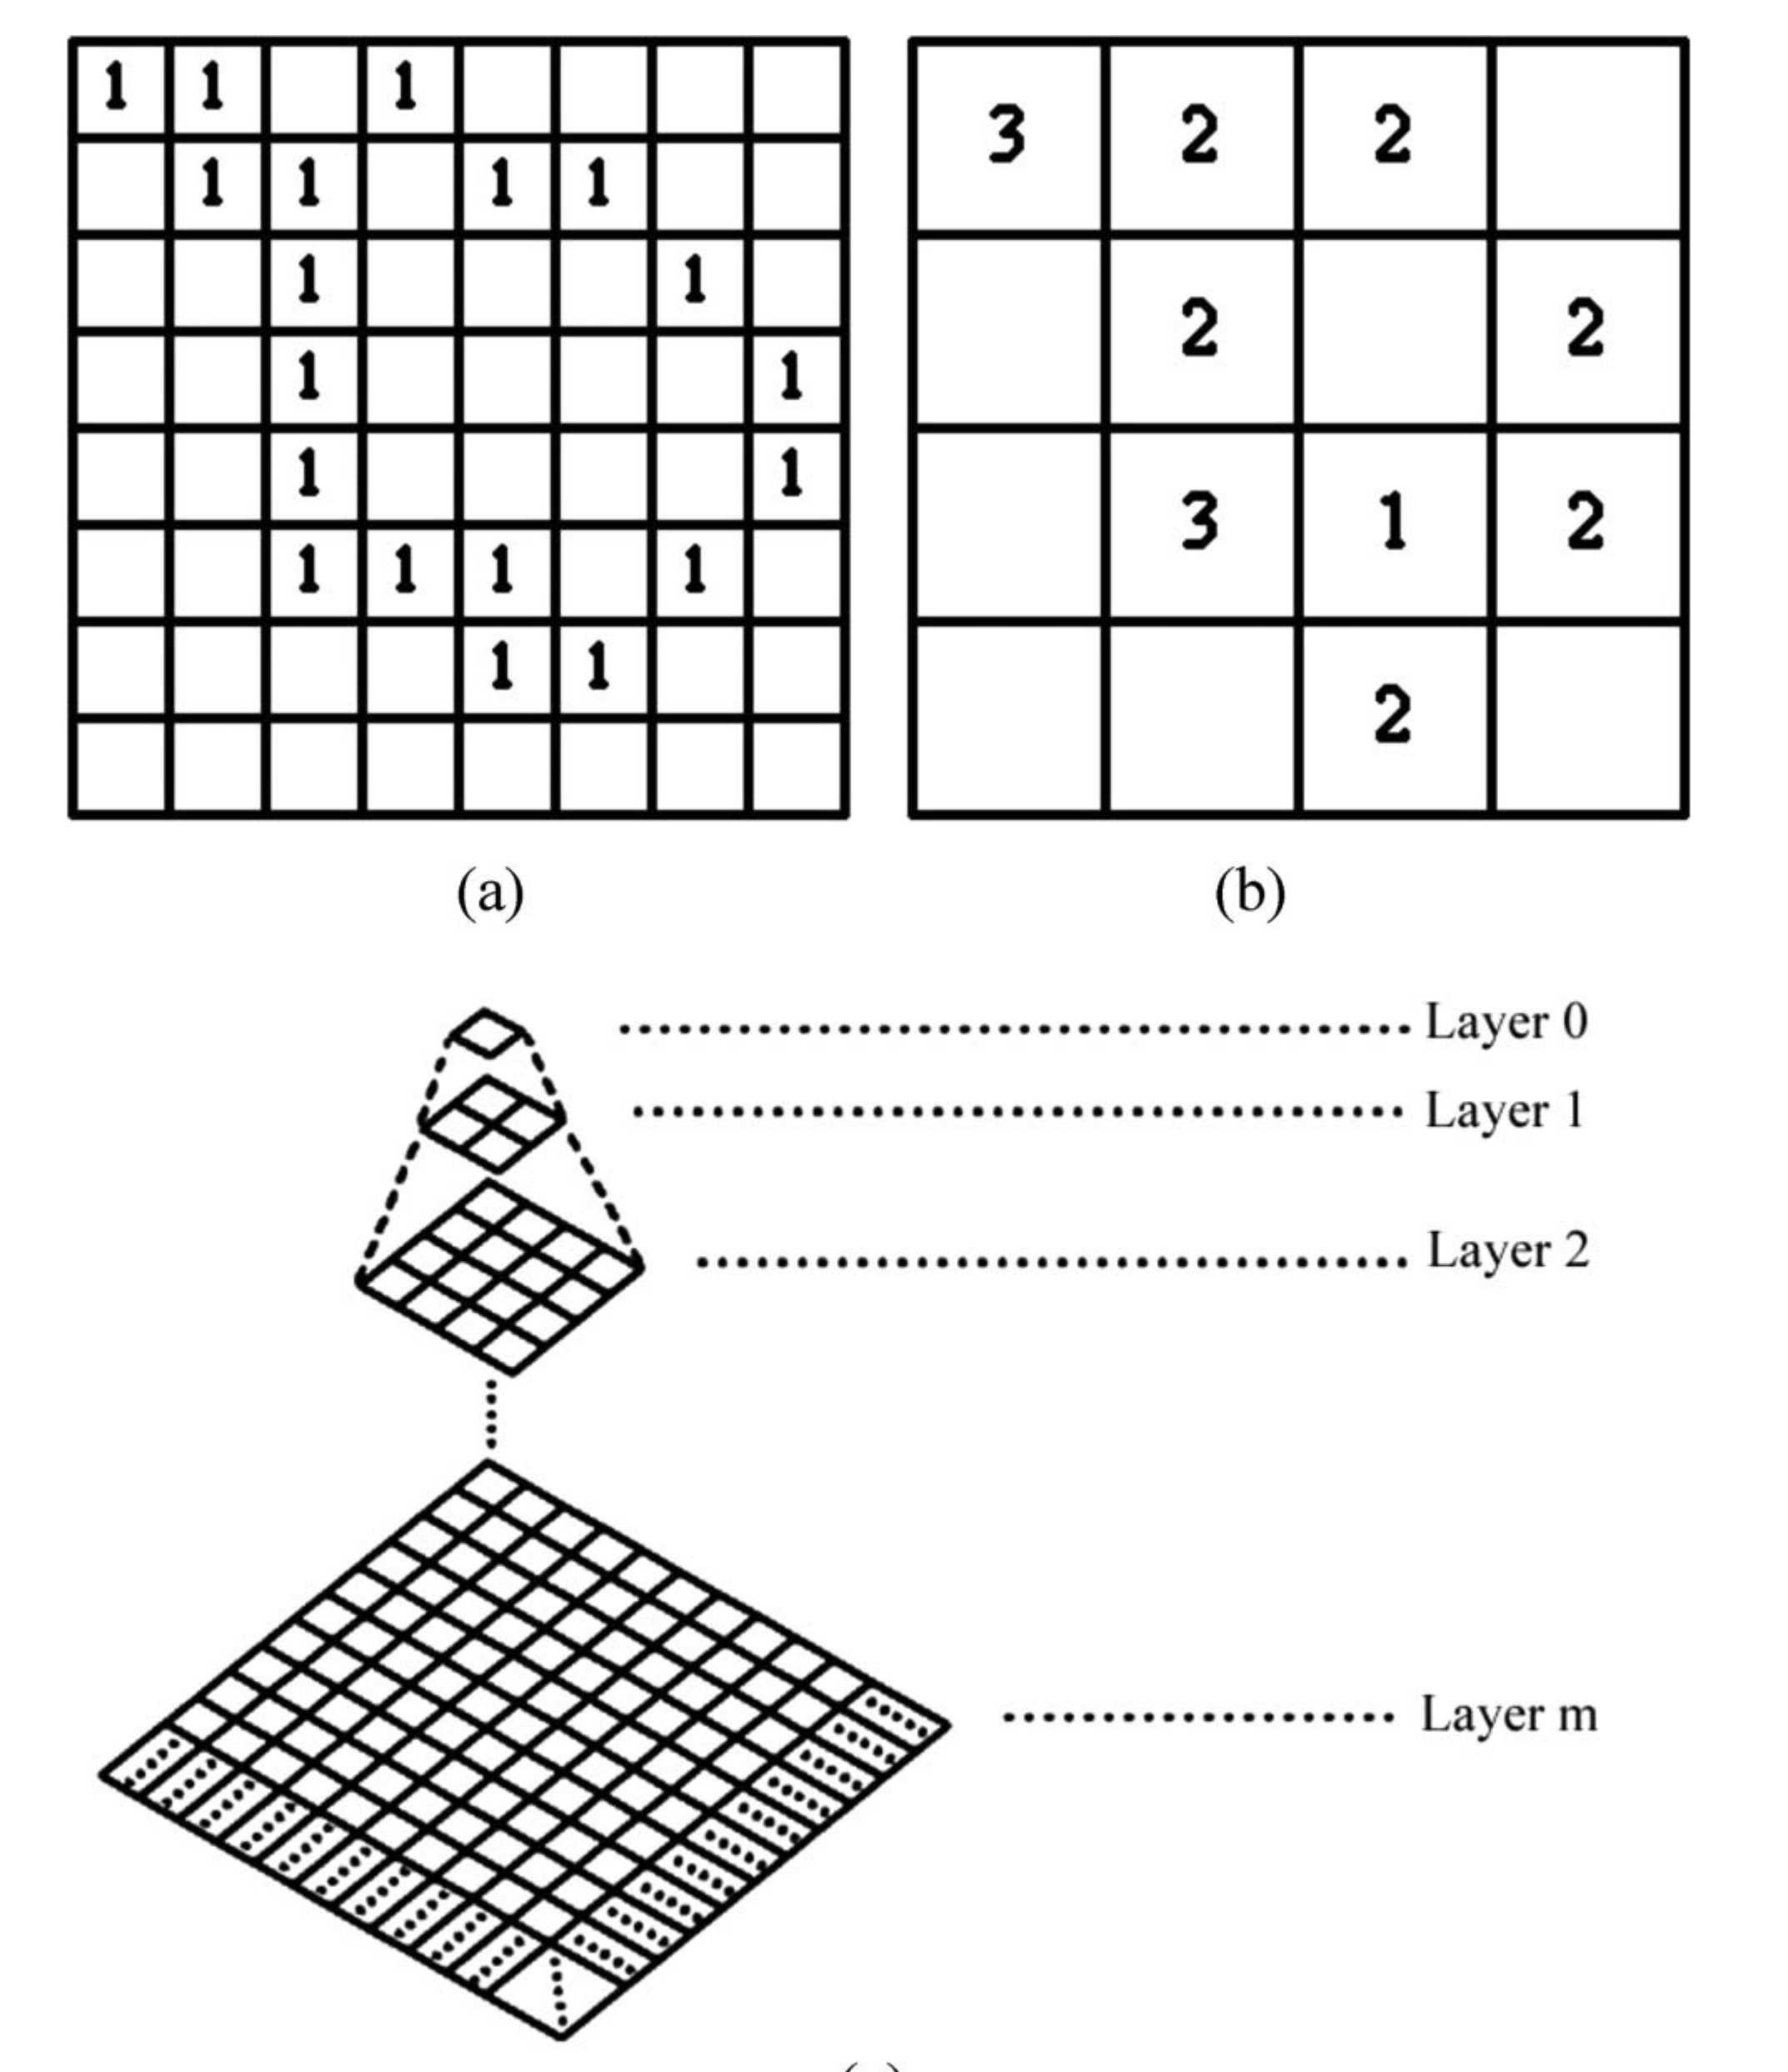
\includegraphics[width=7cm]{elliptic.png}}
\caption{استفاده از هرم تصویر در تبدیل هاف \cite{ellipticalHT} }
\label{fig:elliptic}
\end{figure}


\subsection{روش‌های ابتکاری یا ترکیبی}

یکی از ابتکارات موجود، استفاده از فیلتر کالمن بسط‌ داده‌شده\LTRfootnote{ Extended Kalman Filter (EKF)} است. از آن‌جا که \lr{EKF} یک ابزار ریاضی برای بهبود مدل پیش‌گویانه بر اساس مشاهدات بهبود‌بخش است،‌ به عنوان یک ابزار شهودی در بینایی ماشین استفاده می‌شود\cite{EKF}. جزییات این روش بیشتر شبیه روش‌های برازش بیضی است و کمتر از ایده‌های بینایی ماشین استفاده کرده‌است. 


روش‌های آماری نیز برای تشخیص بیضی استفاده شده‌است. روش‌های مبتنی بر اجماع تصادفی نمونه‌ها\LTRfootnote{ RANdom SAmple Consensus (RANSAC)}\cite{RANSAC} و الگوریتم‌ ژنتیک\cite{GA} به این شکل هستند که تصویر را به زیرمجموعه‌هایی تقسیم می‌کنند. الگوریتم تصادفی، نمونه‌هایی از لبه‌ها را انتخاب می‌کند تا محتمل‌ترین مجموعه پارامتر بیضی را برای آن‌ها تشکیل دهد. سپس یک تابع هزینه برای ارزیابی وجود بیضی استفاده می‌شود که بر مبنای شمارش نقاط در نزدیکی مجموعه‌ی پارامترهای بیضی است و در نهایت یک نتیجه‌گیری برای وجود بیضی انجام می‌شود. هر دوی این الگوریتم‌ها در حضور نویز یا بیضی‌های متعدد، کارایی خود را از دست می‌دهند. برای رفع این مشکلات، شبه \lr{RANSAC}\cite{pRANSAC} و الگوریتم ژنتیک چند جمعیتی\cite{mulGA} ارایه شدند. 

روش دیگر، روش رشد بیضی\LTRfootnote{ Ellipse growing}\cite{grow} نام دارد. این روش بر مبنای تبدیل هاف برای پیدا کردن دایره‌های مماس بر قطعات لبه‌ی موجود در تصویر است و پس از آن، طی یک روال تکراری، این قطعات با کمک اطلاعات تانژانت پیکسل‌های لبه، به بیضی رشد داده می‌شوند. اگر لبه‌ی جدایی تشخیص داده‌شود عملیات متوقف و بیضی تشخیص داده‌شده نادیده گرفته‌می‌شود. تفاوت این روش با روش‌های قبلی در آن است که وقتی نیاز به دقت تقطیع بالا داشته باشیم، این روش با وجود بار محاسباتی زیاد، بهتر عمل می‌کند و در تشخیص بیضی‌های پوشیده‌شده نیز موفق‌تر بوده‌است. 

روش‌های ترکیبی نیز اولین بار در \cite{comb} ارایه شد که از یک تبدیل هاف برای تشخیص مراکز بیضی‌های کاندید کمک گرفته‌شد و با کمک ویژگی‌های هندسی و روش کمترین مجموع مربعات، مراکز نامناسب حذف شدند. 


در \cite{geo}، یک روش مبتنی بر ویژگی‌های هندسی ارایه شده‌است که از قطعات لبه با اشکال خاصی استفاده می‌کند و این قطعات، لبه‌ها را به سه نوع خط، کمان و کمان‌کشیده\LTRfootnote{ Extended arc} تقسیم می‌کند. با ارایه‌ی ویژگی‌های هندسی بیضی، قاعده‌ای برای تشکیل بیضی از این قطعات ارایه شده‌است که در این گزارش به بررسی بیشتر این روش در بخش پنجم خواهیم پرداخت.

\newpage

\section{تبدیل هاف سریع بیضی \lr{(FEHT)}}

در این بخش به بررسی جزیی‌تر روش ارایه‌شده در \cite{FEHT} می‌پردازیم. 

همان‌گونه که در بخش اول گفته شد، تبدیل هاف به روش معمول برای تشخیص بیضی نیاز به فضای پارامتری پنج‌بعدی دارد. بنابراین، این روش از نظر محاسباتی بسیار سنگین می‌شود و از نظر مصرف حافظه نیز کارا نیست. 

یکی از روش‌های کارا برای محاسبه‌ی پارامترها،‌ شکستن پروسه‌ی تشخیص به مراحل کوچک‌تر و استفاده از اطلاعات گرادیان است که کمک می‌کند در هنگام شناسایی شی، یکی از پارامترها را تشخیص دهیم \cite{decompose}. 

از سوی دیگر، الگوریتم‌های تمرکزی وجود دارند که اجازه می‌دهند بیشینه در فضای پارامتر را با محاسبات و مصرف حافظه‌ی کمتری نسبت به روش جست‌وجوی سرکشی\LTRfootnote{ Polling-search} معمول در فضای کامل پارامتر، پیدا کنیم\cite{FHT}. در این میان \lr{FHT} به‌دلیل سادگی محاسبات و قاعده‌مند بودن معمول‌تر از روش‌های دیگر است. هرچند اشکالاتی نیز دارد که ناشی از استراتژیِ دنبال‌شده در آن است و زمانی که تصویر شامل چند شکل با اندازه‌های متفاوت باشد، مشکل‌زا می‌شود. 

در روش ارایه‌شده در \cite{FEHT}، الگوریتم تمرکز جدیدی پیشنهاد شده‌است که مشکلات \lr{FHT} را رفع کرده‌است. با تجزیه‌ی فضای پارامتر و ترکیب آن با این الگوریتم، الگوریتم \lr{FCHT} برای دایره و \lr{FEHT} برای بیضی ارایه‌شده است. این روش برای پیدا کردن مراکز شکل‌ها، حذف جواب‌های نامناسب به محض پیدا شدن برای جلوگیری از دخالت در محاسبات و برای برچسب‌گذاری نقاط شکل‌های مختلف جهت این‌که در مراحل بعدی تنها نقاط اثرگذار در پیدایش همان شکل استفاده‌‌شوند، محاسبات کمتری دارد. 

\subsection{الگوریتم و استراتژی تمرکز}

الگوریتم‌های تمرکز، به دنبال آن نواحی از فضای پارامتر می‌گردند که مقادیر بیشینه‌ را در خود ذخیره کرده‌اند تا بار محاسبات را کمتر کنند. دسته‌ای از این الگوریتم‌ها یک روال تخمین سلسله‌مراتبی را دنبال می‌کنند و در هر گام، بخشی از فضای پارامتر را محاسبه می‌کنند و تصمیم می‌گیرند که به ادامه‌ی تحقیق کردن در این زیرناحیه بپردازند یا خیر. در \lr{FHT} نیز جواب طی یک روال سلسله‌مراتبی تعیین می‌شود که در محل تلاقی چند ابر صفحه قرار دارد. در روش ارایه‌شده، جواب در یک فضای پارامتر دو بعدی خواهد بود که به شرح جزییات آن خواهیم پرداخت. همچنین در این روش، جواب در محل تلاقی دسته‌ای از خطوط خواهد بود. تمرکز به سمت جواب، طی یک پروسه‌ی تقسیم و درج در فضای پارامتر حاصل می‌شود. برای این کار یک مربع در فضای پارامتر ایجاد می‌شود و به چهار قسمت تقسیم می‌شود. هر یک‌چهارم به تعدادی خط قابل ارزیابی (که از مقدار آستانه‌ای بیشتر باشد) که آن‌جا را پیمایش می‌کنند تقسیم می‌شود. تکرار بازگشتی این عمل، جواب را پیدا می‌کند. 

برای یک خط، تصمیم گیری این که آیا از مربع خاصی عبور می‌کند را این‌گونه انجام می‌دهیم که فاصله‌اش با مرکز مربع را حساب می‌کنیم. اگر این فاصله از شعاع دایره‌ی محیطی مربع کم‌تر بود، آن خط این مربع را پیمایش می‌کند. برای این کار تنها نیاز است مرکز مربع، طول ضلع آن و ضرایب توصیف‌کننده‌ی خط را بدانیم. در ادامه خواهیم دید این ضرایب، مختصات نقاط در تصویر و بردارهای گرادیان متناظرشان خواهد بود. عبارتی که فاصله‌ی یک خط به معادله‌ی 
\( A_{2}y + A_{1}x + A_{0} = 0 \)
را از مربع 
\( c= (c_x , c_y) \)
می‌دهد به این شکل است: 
\begin{equation}
\label{eq:focus}
d_c = A_{2}c_y + A_1 c_x + A_0
\end{equation}
که در آن اندازه‌های ضرایب به‌گونه‌ای نرمال شده‌است که 
\( (A_2)^2 + (A_1)^2 = 1 \) 
باشد. معادله‌ی \lr{FHT} به‌گونه‌ای است که پس از محاسبه‌ی فاصله تا مرکز یک مربع، فاصله تا یک‌چهارم‌های آن مربع با عملیات کاهش‌یافته‌ی جمع و شیفت قابل محاسبه‌ است. از سوی دیگر برای کاهش محاسبات، یک بردار حضور\LTRfootnote{ Presence vector} تشکیل می‌شود که نشان می‌دهد هر خط در فضای پارامتر، کدام یک‌چهارم را پیمایش می‌کند (یک بیت از بردار به ازای هر خط).

استراتژی تمرکز مشخص می‌کند که چگونه یک‌چهارم‌ها را تقسیم کنیم و درخت ایجادشده را چگونه بررسی کنیم. استراتژی اول سطح، حافظه‌ی زیادی مصرف می‌کند و از طرفی، چون قاعده‌ی خاصی برای مشخص کردن این‌که کدام نود بهتر است باز شود نداریم، حرکت به سوی جواب ممکن است کند باشد. استراتژی اول عمق، کمی بهبود حاصل می‌شود اما همچنان نداشتن قاعده برای انتخاب بهترین نود از نودهای کاندید برای بسط دادن، کارایی را کم می‌کند. یکی از بهبودهای پیشنهادی این است که نودی که تعداد خط بیشتری را شامل شده‌است انتخاب شود که این کار در مواردی که چندین جواب در فضای پارامتر موجود است، ممکن است فشار انتخاب یک جواب را بالا ببرد. 

برای حل مشکلات مطرح در استراتژی، یک الگوریتم تمرکز جدید معرفی شده‌است که بهترین عمق و سطح را انتخاب می‌کند. با شروع از سطح اول، همه‌ی نودهای ممکن تولید می‌شوند، ولی تنها نودهایی بررسی می‌شوند که از حاصل‌ضرب مقدار بیشینه با یک ضریب معین که ضریب تمییز\LTRfootnote{ Discrimination factor} نامیده می‌شود، بیشتر باشند. 

\subsection{تشخیص بیضی}

نقاط روی یک بیضی، در رابطه‌ی زیر صدق می‌کنند: 
\begin{align}
{{ [ (x_p - x_0 ) \cos\phi + (y_p - y_0 ) \sin\phi ]^2 } \over {a^2} } + { { [ (x_p - x_0 ) \sin\phi - (y_p - y_0 ) \cos\phi ]^2 } \over {b^2} }= 1
\end{align}
که در آن
\( x_0 \) 
و 
\( y_0 \) 
مختصات مرکز،
\( \phi \) 
زاویه‌ی جهت و 
\( a \)
و 
\( b \)
نیم‌قطرها هستند. به جای استفاده از روش معمول در \lr{FHT} که نیاز به یک فضای پنج‌بعدی دارد و حافظه‌ی زیادی مصرف می‌کند و پردازش سنگینی دارد، از اطلاعات بردار مشتق استفاده شده‌است تا محاسبه‌ی پارامترها به چند مرحله شکسته‌شود. مراحل ارایه‌شده به این شکل است: 
\begin{enumerate}
\item 
تشخیص مرکز با استفاده از الگوریتم تمرکزی که نقطه‌ای را پیدا می‌کند که در آن دسته‌ای از خطوط هم را قطع می‌کنند.

\item
تولید زاویه‌ی 
\( \phi \) 
و نرخ 
\( a^2/b^2 \) 
با توجه به اطلاعات مرحله‌ی قبل و بردار گرادیان شکل‌ها. 

\item 
محاسبه‌ی نیم‌قطرهای 
\( a \)
و 
\( b \)
از معادله‌ی بیضی. 

\end{enumerate}


\subsubsection{تشخیص مراکز}
\label{subsec:centers}
%\begin{wrapfigure}{l}{0.5\textwidth}
%   \vspace{-2cm}
%  \begin{center}
\begin{figure}[h]
\centering
\frame{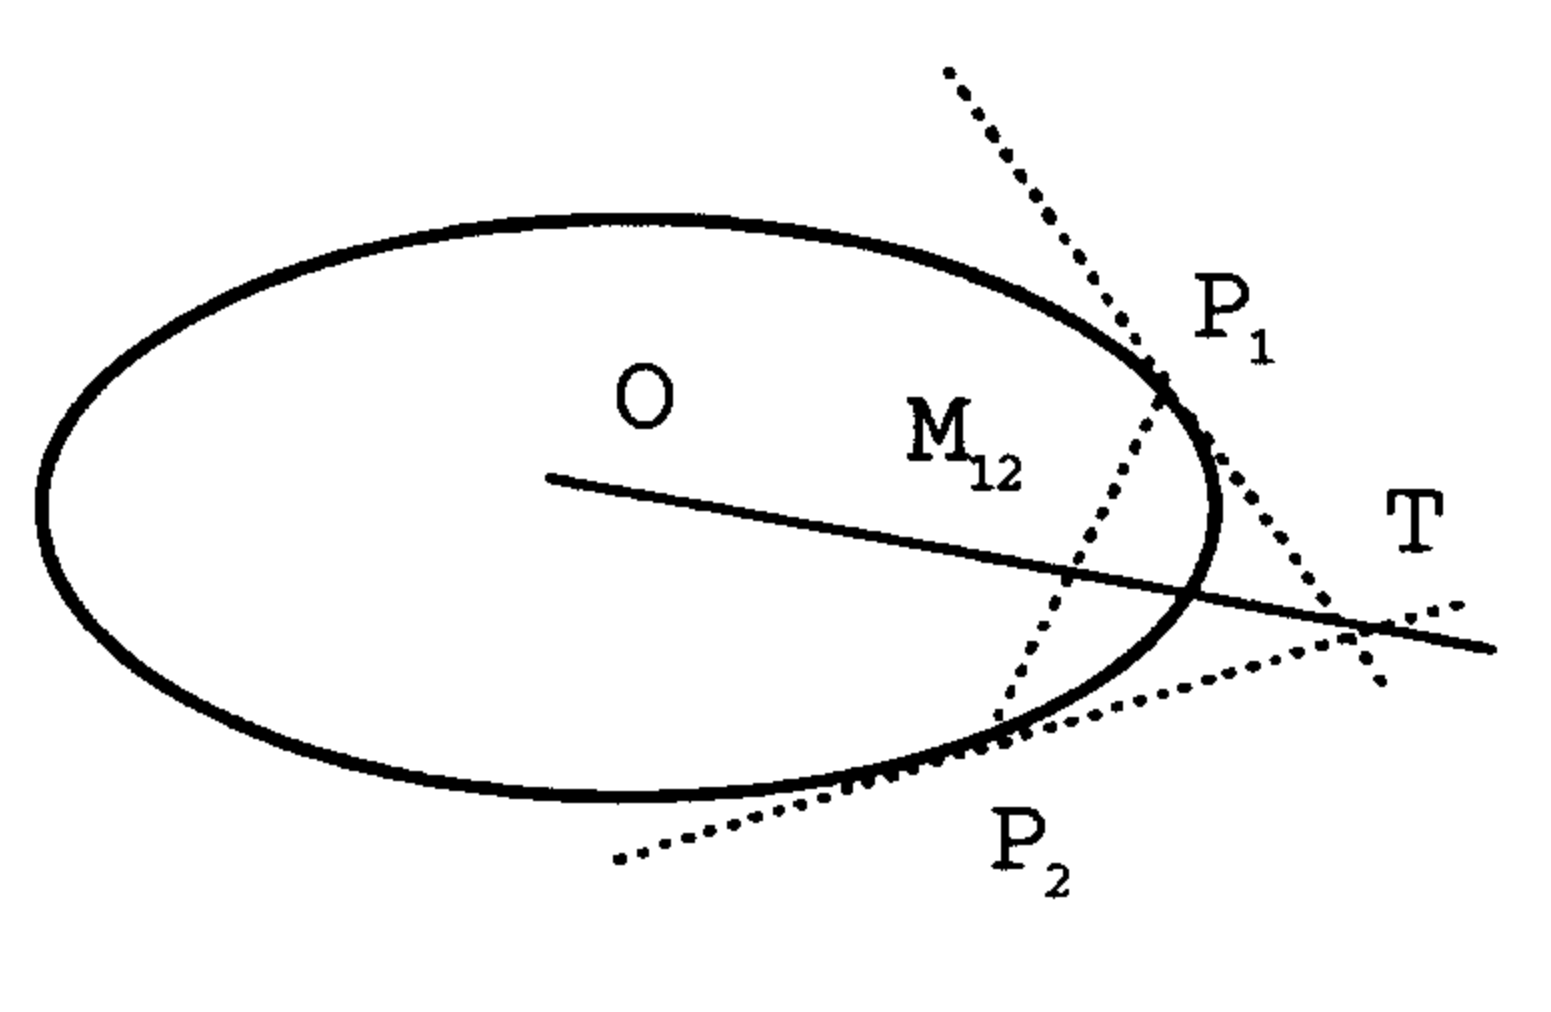
\includegraphics[width=6cm]{fig8.png}}
\caption{تولید دسته‌ای از خط‌ها برای بیضی \cite{FEHT} }
\label{fig:lineBeam}
%\end{center}
\end{figure}
%\end{wrapfigure}

با فرض این‌که 
\( P_1 = (x_1,y_1) \)
و
\( P_2= (x_2,y_2) \)
دو نقطه از بیضی با شیب‌های\LTRfootnote{ Slope} 
\( \xi_1 \)
و 
\( \xi_2 \)
باشند،‌ که در نقطه‌ی 
\( T_{12} \) 
که در شکل \ref{fig:lineBeam} نشان‌داده شده‌است، یکدیگر را قطع می‌کنند. خطی که نقطه‌ی 
\( T_{12} \) 
و نقطه‌ی وسط
\( M = [ (x_1 + x_2)/2 , (y_1+y_2)/2 ] \) 
می‌گذرد، از مرکز بیضی عبور می‌کند. 

بنابراین با استفاده از جفت نقاطی که شیب‌های موازی ندارند می‌توان دسته‌ای از خطوط تولید کرد که هم را در مرکز بیضی قطع می‌کنند. با اعمال الگوریتم \lr{FHT} بر روی این فضا، مرکز بیضی به‌دست می‌آید. در این مرحله هر خط با ضرایب نرمال‌شده‌ی متناظر با معادله‌ی \ref{eq:focus} تعریف می‌شود: 

\begin{align}
A_0^{p_1 p_2} = {{t_1 m_2 - t_2 m_1} \over { \Gamma_{12} }} 
\hspace*{0.2cm}, \hspace*{0.2cm}
A_1^{p_1 p_2} = {{t_2 - m_2} \over { \Gamma_{12} }} 
\hspace*{0.2cm}, \hspace*{0.2cm} 
A_2^{p_1 p_2} = {{t_1 - m_1} \over { \Gamma_{12} }}
\end{align}
\label{eq:coefs}

که در آن: 

\begin{gather}
\begin{align*}
t_1 = { {y_1 - y_2 - x_1 \xi_1 + x_2 \xi_2 } \over {\xi_2 - \xi_1 } } 
\hspace*{0.2cm},& \hspace*{0.2cm}
t_2 = { { \xi_2 \xi_1 (x_2 - x_1) - {y_2 \xi_1} + {y_1 \xi_2} } \over {\xi_2 - \xi_1 } }, \nonumber 
\\[0.5cm]
m_1 = {{x_1 + x_2} \over 2}
\hspace*{0.5cm},& \hspace*{0.5cm}
m_1 = {{y_1 + y_2} \over 2} ,
\end{align*}
\\[0.5cm]
\Gamma_{12} = \sqrt{(t_2 - m_2)^2 + (t_1 - m_1 )^2 }
\label{eq:coefsParams}
\end{gather}

شیب نقاط از اطلاعات گرادیان در آن‌ها به‌دست می‌آید. به این صورت، اگر 
\( \theta \) 
زاویه‌ی گرادیان در نقطه‌ی
\( P \) 
باشد، زاویه‌ی گرادیان در آن نقطه برابر است با: 
\begin{equation}
\label{eq:gradTg}
\xi_p = \theta_p - { \pi \over 2}
\end{equation}

به این ترتیب می‌توان با پیچیدگی زمانی برابر 
\( O(n^2) \)
مرکز بیضی‌ها را پیدا کرد. جزییات پیچیدگی زمانی برای هر بخش و نیز شروط انتخاب نقاط در شرایط خاص در \cite{FEHT} آمده‌است که بیان آن از حوصله‌ی این بخش خارج است.
\\
\\
\subsubsection{تشخیص جهت‌ها}

با محاسبه‌ی مشتقات جزیی معادله‌ی بیضی بدون دوران، هر نقطه‌ی 
\( P \) 
روی کانتور بیضی در معادله‌ی زیر صدق می‌کند:

\begin{equation}
{ a^2 \over b^2} = { (x_p - x_0) \over (y_p - y_0)} \tan \theta_p 
\label{eq:deriv}
\end{equation}

اگر بیضی به اندازه‌ی 
\( \phi \)
دوران داده‌ شده‌باشد، معادله‌ی \ref{eq:deriv} به این صورت درمی‌آید: 

\begin{equation}
{ a^2 \over b^2} = { {(x_p - x_0) \cos \phi + (y_p - y_0 ) \sin \phi} \over {(x_p - x_0)\sin \phi - (y_p - y_0 ) \cos \phi}} \tan (\theta_p - \phi )
\label{eq:derivPhi}
\end{equation}

با توجه به آن‌که مختصات مراکز را از مرحله‌ی قبل به‌دست آورده‌ایم، در این بخش می‌توانیم از یک فضای دو بعدی استفاده کنیم که درآن هر نقطه از بیضی برای جهتی خاص رای می‌دهد. پس از آن که مقادیر بیشینه را پیدا کردیم، جهات مختلف بیضی‌ها در تصویر را به‌دست آورده‌ایم و با توجه به معادله‌ی \ref{eq:derivPhi}، نسبت نیم‌قطرها نیز به‌دست می‌آید. 

باید به این نکته دقت داشت که برای صرفه‌جویی در استفاده از توان پردازشی، در این فاز تنها از نقاطی استفاده می‌شود که در پیدا کردن مراکز بیضی‌ها نقش داشته‌اند. به همین ترتیب اگر بیضی‌های هم‌مرکز ولی با جهات متفاوت وجود داشته باشد، در این فاز رای‌گیری نقاطی که در پیدا کردن یک مرکز مشترک مشارکت داشته‌اند، هم‌اکنون به جهات و نرخ‌های نیم‌قطرهای متفاوت رای می‌دهند. 

\subsubsection{تشخیص نیم‌قطرها}

برای همه‌ی نقاطی که در مرحله‌ی قبل مشارکت کرده‌اند، دورانی به اندازه‌ی 
\( \phi \) 
انجام داده‌می‌شود و به‌جای نرخ نیم‌قطرها، 
\( h \) 
قرار داده‌می‌شود. پس مقادیر نیم‌قطرها به این‌گونه به‌دست می‌آید: 

\begin{gather}
b = \sqrt{h^{-1}(x_p - x_0)^2 - (y_p-y_0)^2}
\nonumber
\\[0.5cm]
a = \sqrt{(x_p - x_0)^2 + h(y_p-y_0)^2}
\label{eq:semiaxis}
\end{gather}
در این‌جا نیز برای کاهش پیچیدگی می‌توان از این نکته سود برد که نقاطی که در فاز پیش رای داده‌اند به نسبت خاصی از مقادیر نیم‌قطرها رای داده‌اند و در پیدا کردن بیشینه‌ها این مطلب برای پیدا کردن زوج‌ نیم‌قطرهای نظیر، مفید است. 

\subsubsection{نتیجه‌گیری}

برای یک تصویر 
\( 512 \times 512 \) 
نزدیک به
\( 50\% \)
از نقاط در روند اجرا حذف شده‌اند. برای لبه‌یابی از عملگر سوبل استفاده شده‌است و ضریب تمییز برابر با 
\( 0.8 \) 
قرارداده شده‌است. 


\begin{figure}[h]
\centering
\frame{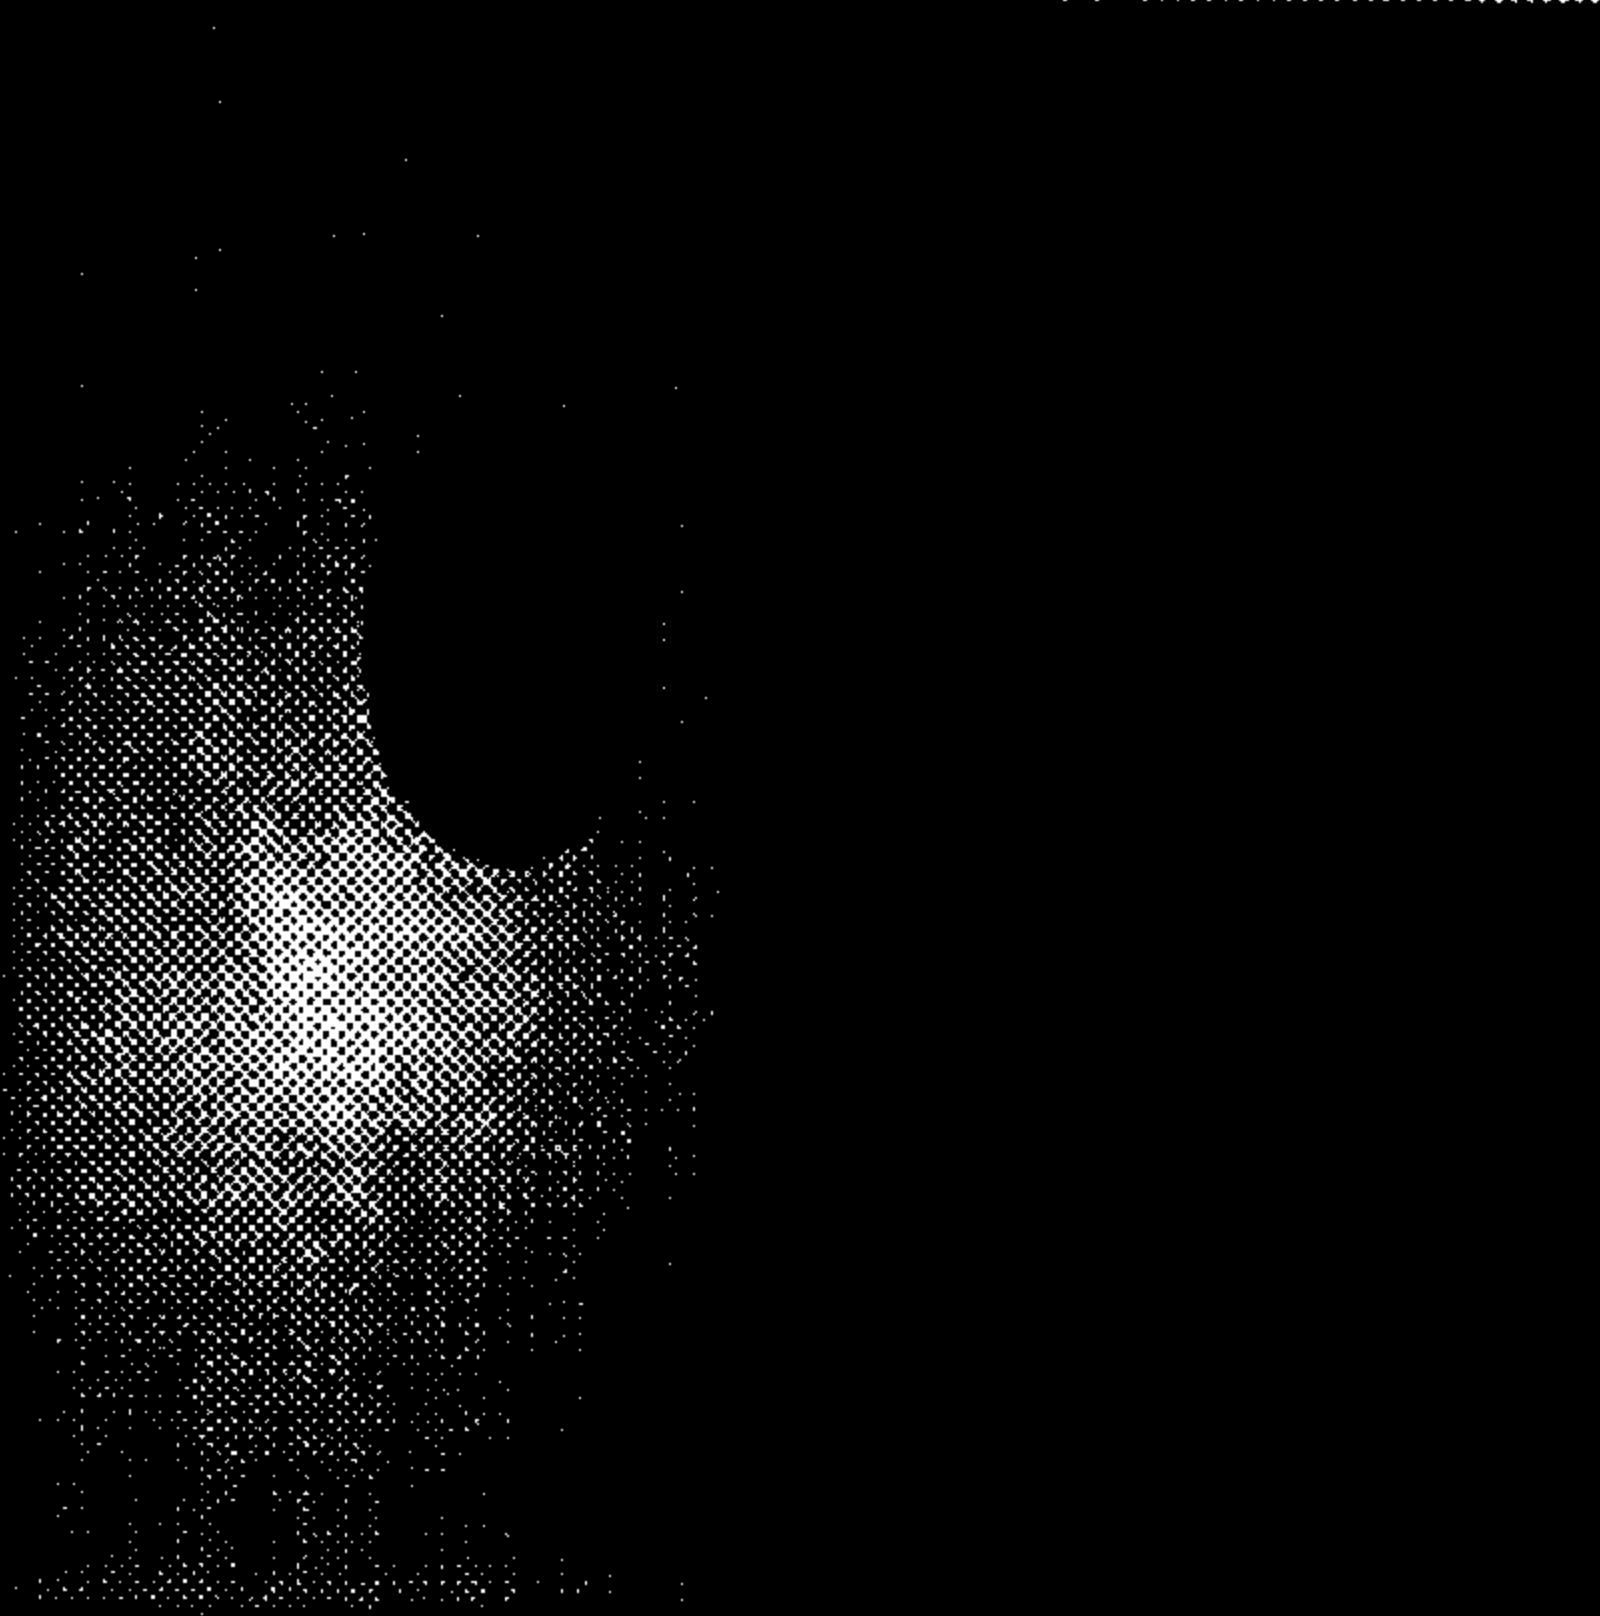
\includegraphics[height=6cm]{ell1.png}}
\hspace{3mm}
\frame{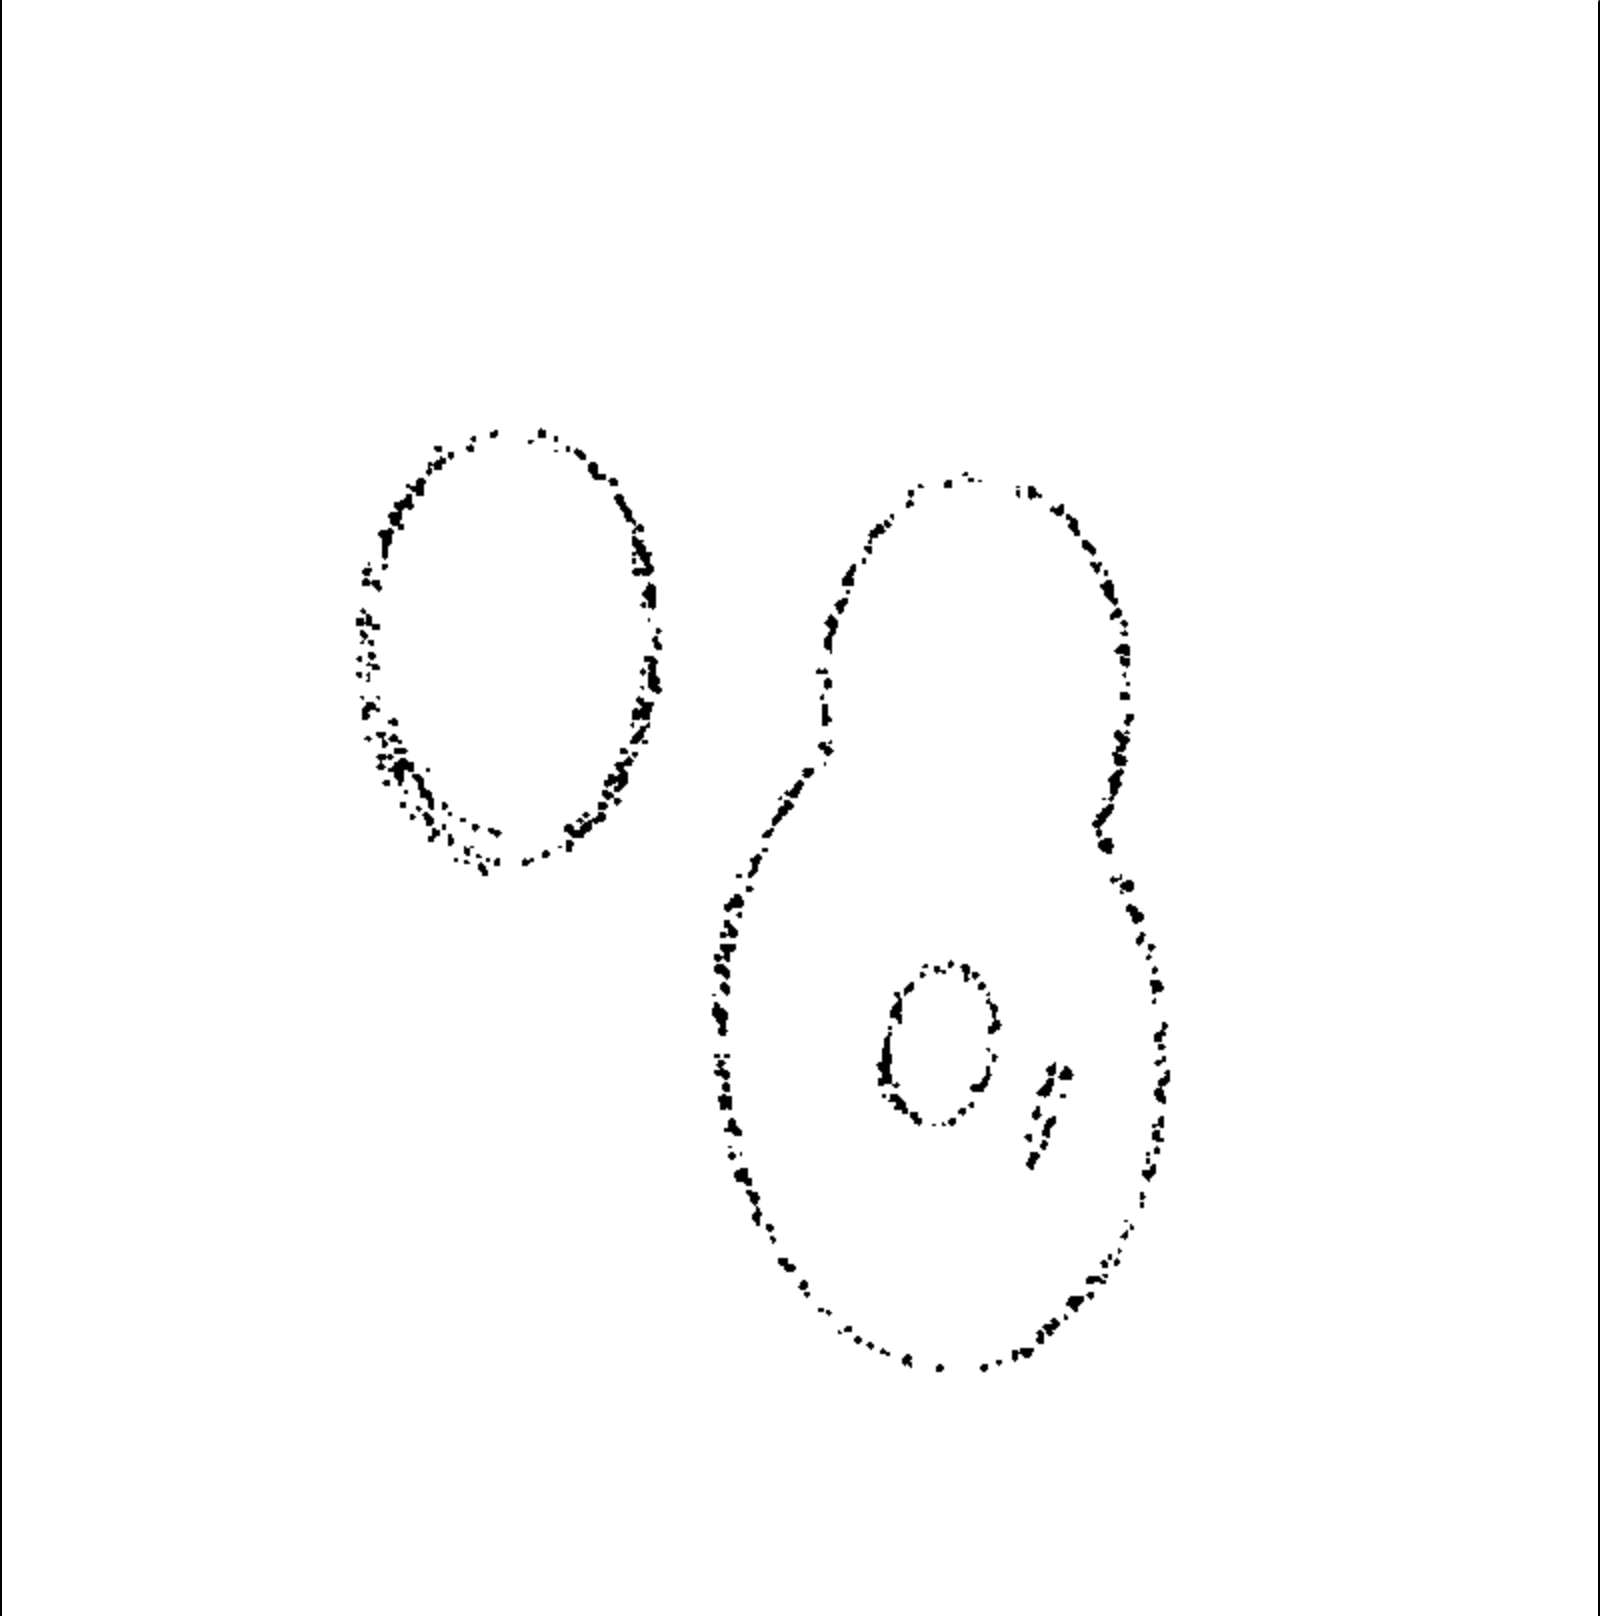
\includegraphics[height=6cm]{ell2.png}}
\caption{راست: تصویر اصلی. چپ: تصویر لبه‌یابی‌شده \cite{FEHT} }
\label{fig:fehtMain}
\end{figure}

\begin{figure}[h]
\centering
\frame{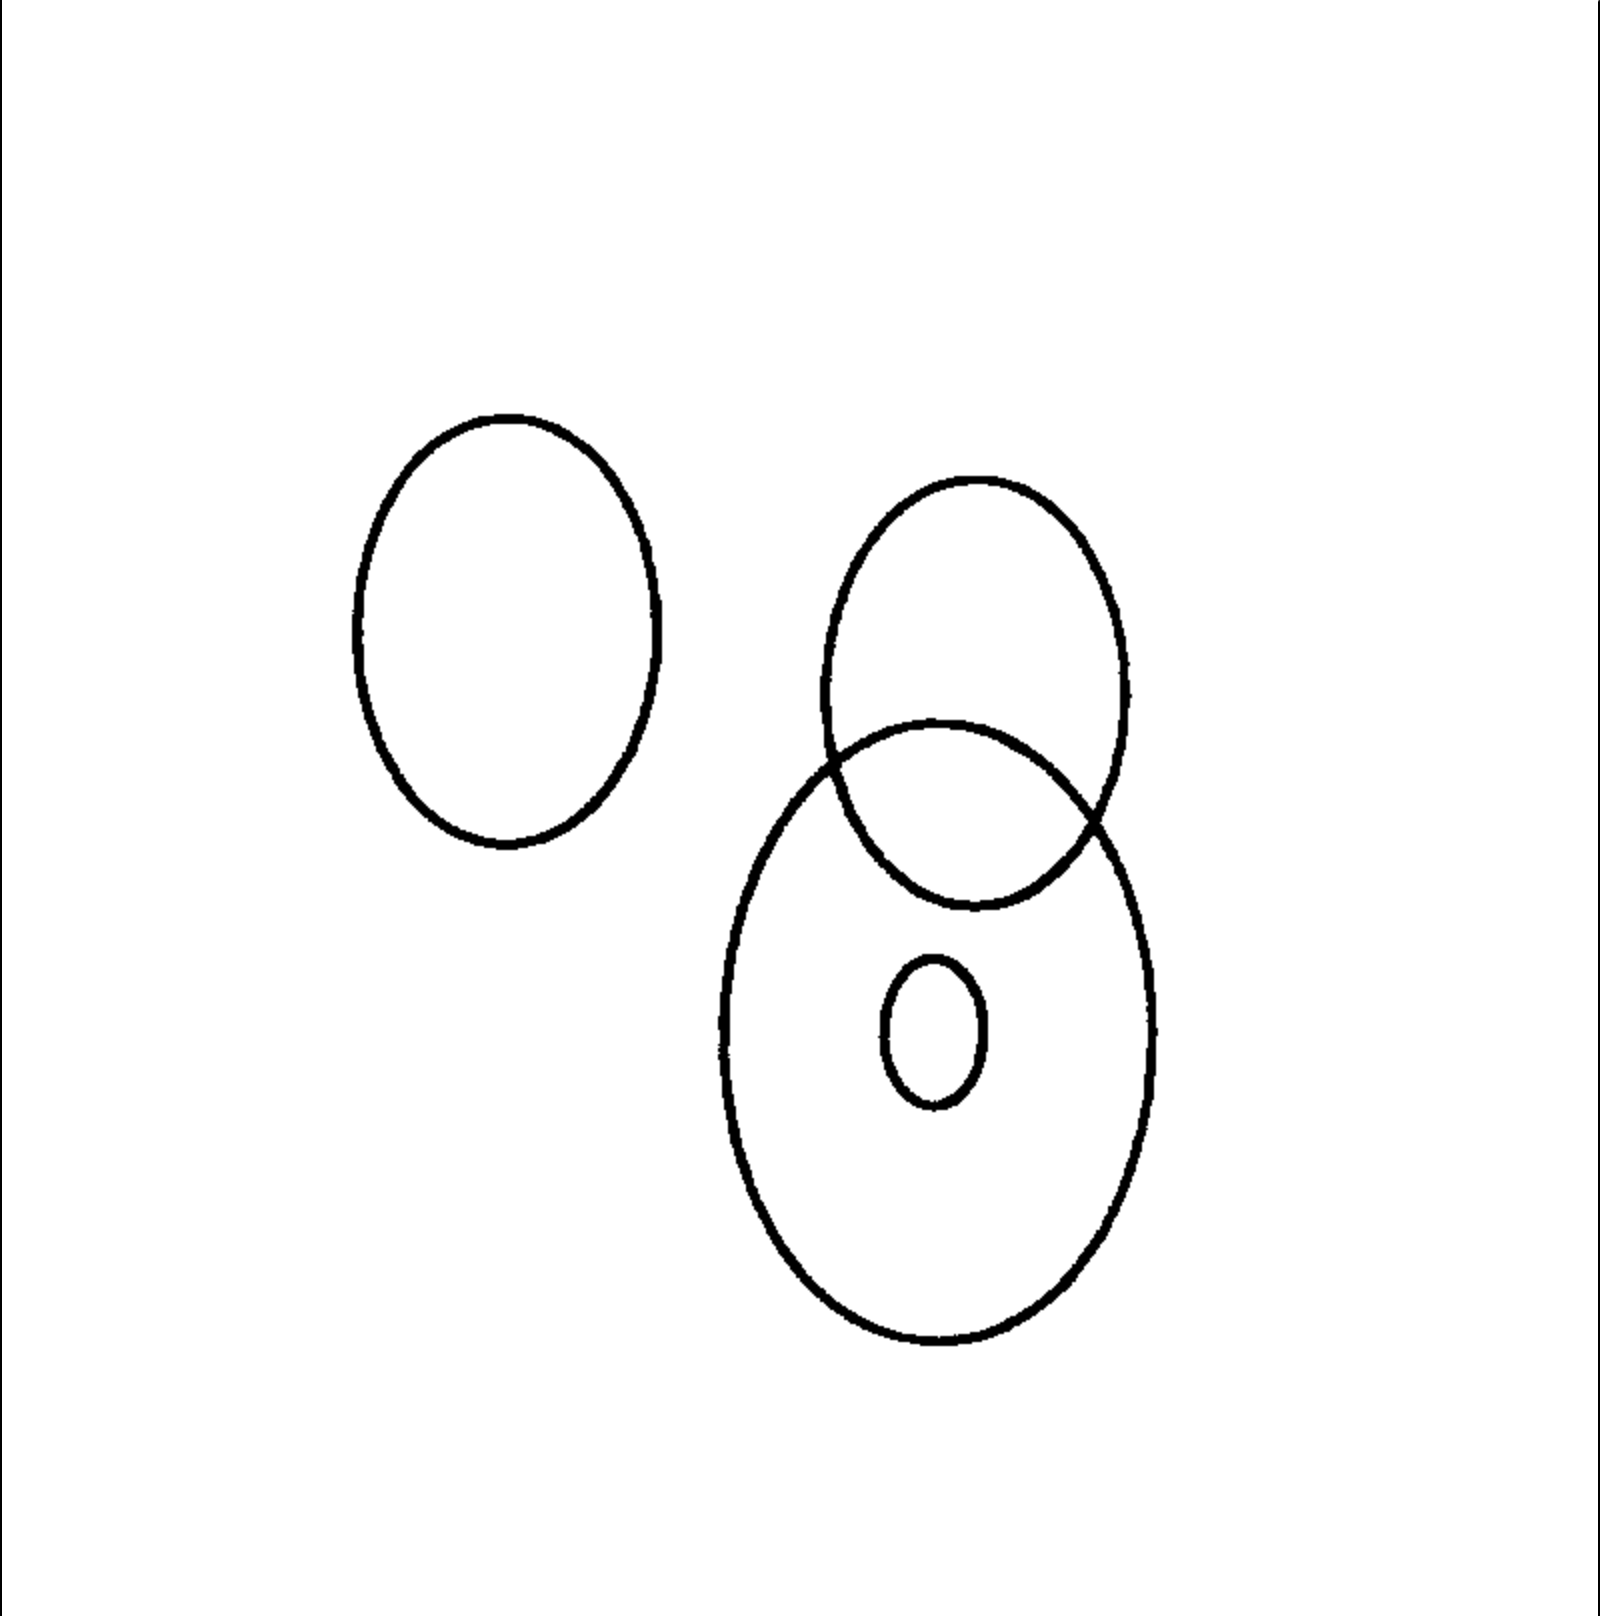
\includegraphics[height=6cm]{ell3.png}}
\caption{بیضی‌های تشخیص داده‌شده \cite{FEHT}}
\label{fig:fehtDetect}
\end{figure}

طبق آزمایشات \cite{FEHT}، این روش در مقایسه‌ با هاف بیضی در جدول \ref{tab:feht} مقایسه شده‌است. تعداد نودها، حداکثر تعداد نودهای قابل بررسی در استراتژی تمرکز است.

\vspace{0.7cm}
\begin{table}
\centering
\begin{tabular}{r@{\hskip 1cm}r@{\hskip 1cm}r@{\hskip 1cm}}
\hline\noalign{\smallskip}
نودهای & زمان  & افزایش \\
فعال & \lr{(s)} & سرعت\lr{(\%)}
\\[0.2cm]
\hline\noalign{\smallskip}
\(4\) & \(100\) & \(0\)\\[0.2cm]
\(8\) & \(71\) & \(29\)\\[0.2cm]
\(12\) & \(79\) & \(21\)\\[0.2cm]
\(16\) & \(75\) & \(25\)\\[0.2cm]
\hline\noalign{\smallskip}
\end{tabular}
\caption{مقایسه‌ی کارایی با هاف بیضی}
\label{tab:feht}
\end{table}


\newpage

\section{تبدیل هاف تصادفی‌شده برای بیضی \lr{(RHT)}}

یک‌سال پس از ایده‌ی \cite{FEHT}، بهبود دیگری برای استفاده از هاف در تشخیص بیضی انجام گرفت که بر پایه‌ی هاف تصادفی‌شده \cite{RHT-old} طراحی شد \cite{RHT}. برای استفاده از \lr{RHT} باید شکل با یک معادله‌ی خطی توصیف شود، در ادامه به بررسی \lr{RHT} می‌پردازیم و سپس ایده‌ی ارایه‌شده برای توصیف بیضی با یک معادله‌ی خطی را بررسی می‌کنیم. 

روش \lr{RHT}، نقاط را در فضای پارامتر با انتخاب کردن لیست‌های 
\( n\)
تایی از پیکسل‌های تصویر و محاسبه‌ی پارامترهای شکل عبورکننده از آن‌ها، روی‌هم جمع می‌کند.

بیضی با معادله‌ی زیر تعریف می‌شود: 

\begin{equation}
a(x-p)^2 + 2b(x-p)(y-p) + c(y-q)^2 = 1
\label{eq:ellip-rht}
\end{equation}

با این محدودیت که:
\begin{equation}
ac - b^2 > 0
\label{eq:const}
\end{equation}
این معادله غیرخطی است \cite{RHT}.

\subsection{خطی‌سازی}

برای خطی‌سازی روش زیر ارایه شده‌است: 

با انتخاب سه پیکسل از تصویر، تانژانت در آن نقاط محاسبه می‌شود. این کار با تعریف یک همسایگی کوچک در اطراف نقطه و پیدا کردن بهترین خط منطبق به آن پیکسل‌ها (با روش کمترین مربعات) انجام می‌شود.
سه پیکسل
\( x_1 \)،
\( x_2 \)،
\( x_3 \)
و تانژانت محاسبه‌شده، ورودی‌های الگوریتم هستند. 
محاسبه‌ی پارامترهای بیضی به دو مرحله تقسیم می‌شود: پیدا کردن مراکز، و پیدا کردن سه پارامتر دیگر. 

برای پیدا کردن مراکز از روش \cite{rht-cent} استفاده شده‌است که بر اساس ویژگی‌های هندسی بیضی است. به این ترتیب که دو نقطه روی بیضی را در نظر گرفته و نقطه‌ی میانی آن‌ها 
\(m\)
نامیده می‌شود. همچنین محل تلاقی تانژانت‌های آن‌ها 
\( t \)
نامیده می‌شود. مرکز بیضی بر روی خط 
\( \widebar{tm} \) 
قرار خواهد داشت. این روش را در شکل \ref{fig:lineBeam} نیز مشاهده نمودیم. به همان روشی که در بخش \ref{subsec:centers} نشان‌ داده‌شد استفاده شده‌است. 

سه پارامتر باقی‌مانده به این روش تخمین‌زده می‌شوند که معادله‌ی \ref{eq:ellip-rht} به این صورت کاهش می‌یابد: 
\begin{equation}
ax^2+2bxy+cy^2 = 1
\label{eq:reduced}
\end{equation}

به این ترتیب با در نظر گرفتن مختصات سه نقطه، سه معادله‌ی خطی داریم:
\begin{equation}
\left[ 
\begin{array}{ccc}
x_1^2 & 2x_1y_1 & y_1^2 \\[0.2cm]
x_2^2 & 2x_2y_2 & y_2^2 \\[0.2cm]
x_3^2 & 2x_2y_2 & y_3^2 \\[0.2cm]
\end{array}
\right]
\left[ 
\begin{array}{ccc}
a \\[0.2cm]
b \\[0.2cm]
c \\[0.2cm]
\end{array}
\right]
=\left[ 
\begin{array}{ccc}
1 \\[0.2cm]
1 \\[0.2cm]
1 \\[0.2cm]
\end{array}
\right]
\label{eq:linear}
\end{equation}

حل این دستگاه معادلات، سه پارامتر باقی‌مانده به دست می‌آیند. اگر بیضی معتبر باشد، پارامترهای به‌دست‌آمده در محدودیت \ref{eq:const} صدق می‌کنند. در غیر این صورت، یا سه نقطه بر روی بیضی قرار ندارند و یا تخمین تانژانت دقیق نبوده‌است. در این صورت سه پیکسل جدید انتخاب می‌شود و الگوریتم ادامه پیدا می‌کند. 

این روش در برابر نویز و تعداد زیاد بیضی در تصویر مقاوم است. نتایج الگوریتم با سه روش دیگر،
\lr{SHT} \cite{PHT}، 
\lr{PHT} \cite{rht-cent}،
\lr{GSHT} \cite{GSHT}
در شکل \ref{fig:rht-c1} آورده شده‌است. 


\begin{figure}[h]
\centering
\begin{subfigure}{0.5\textwidth}
  \centering
  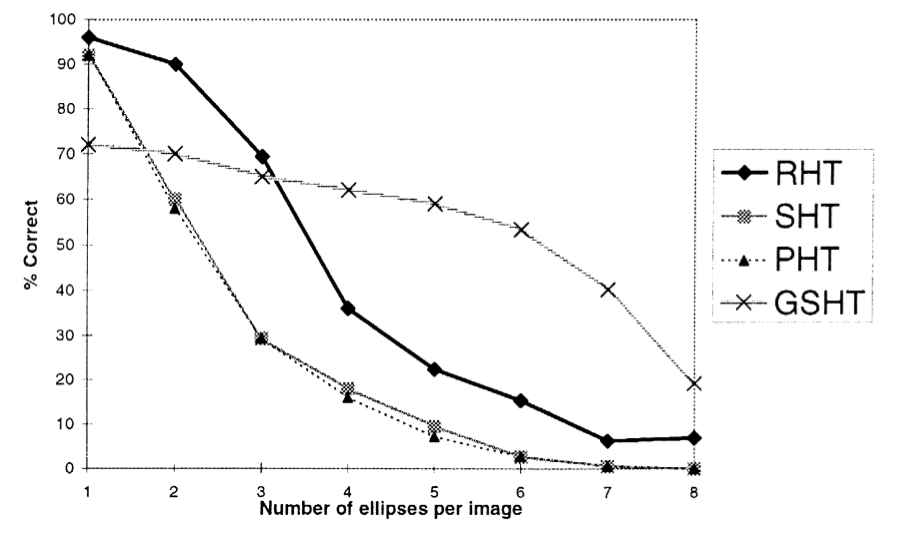
\includegraphics[width=6.8cm]{rht1.png}
  \caption{درصد دقت با چند بیضی}
  \label{fig:rht1}
\end{subfigure}%
\begin{subfigure}{0.5\textwidth}
  \centering
  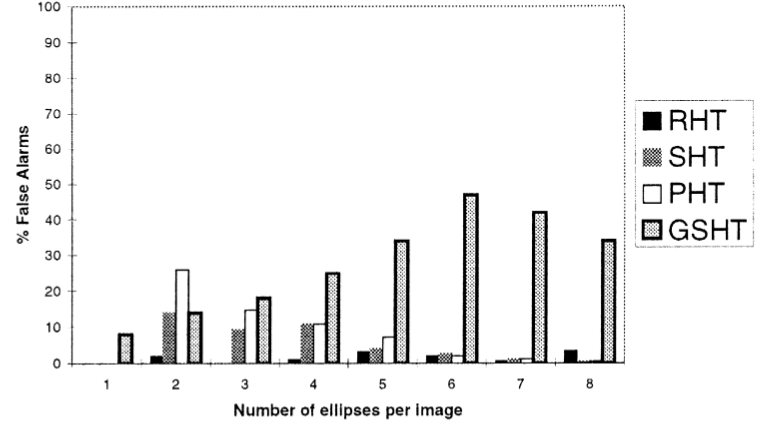
\includegraphics[width=6.8cm]{rht2.png}
  \caption{درصد تشخیص غلط}
  \label{fig:rht2}
\end{subfigure}
\caption{مقایسه‌ی دقت و تشخیص غلط \cite{RHT}}
\label{fig:rht-c1}
\end{figure}

در \cite{cluster} بر مبنای همین روش، بیضی‌ها تشخیص داده‌می‌شوند و با خوشه‌بندی، برای هر دسته بیضی با پارامترهای شبیه، یک بیضی نماینده انتخاب می‌شود که در تشخیص بیضی در تصاویر طبیعی کاربرد دارد.


\newpage

\section{تشخیص بر مبنای ویژگی‌های هندسی}

در \cite{geo} روشی برای تشخیص بیضی بر مبنای ویژگی‌های هندسی و بدون استفاده از تبدیل هاف ارایه شده‌است که نسبت به روش‌های مبتنی بر هاف، حافظه‌ی کمتری مصرف می‌کند. این روش تصویر لبه‌ها را دریافت می‌کند و در چهار مرحله بیضی‌ها را تشخیص می‌دهد. در مرحله‌ی اول قطعات کوچک خط را استخراج می‌کند و در مرحله‌ی دوم با ترکیب این خطوط، کمان‌های کوچک را تشخیص می‌دهد و سپس با ترکیب این قطعات در مرحله‌ی سوم، خم‌های‌کشیده را تشکیل می‌دهند که برای تشخیص بیضی مورد استفاده قرار می‌گیرند. 

\begin{figure}[h]
\centering
\frame{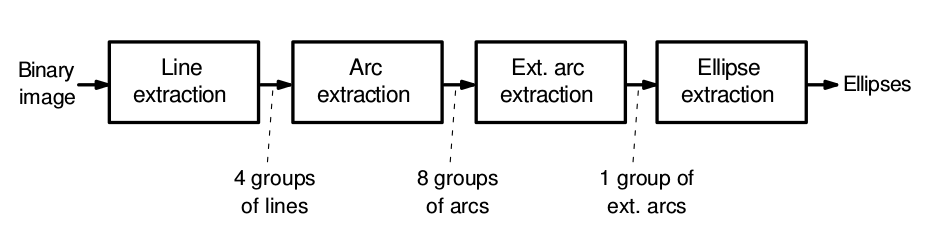
\includegraphics[width=10cm]{4stage.png}}
\caption{مراحل تشخیص در \cite{geo}}
\label{fig:4stage}
\end{figure}
برای تشخیص، از شکل‌ها معرفی‌شده در شکل \ref{fig:segs} استفاده شده‌است. از ترکیب گروه‌های خط و کمان که در شکل \ref{fig:groups} آورده شده‌اند، اشکال یادشده ساخته می‌شوند و با شرط تجاوز نکردن از زاویه‌ی آستانه‌ای، به هم می‌پیوندند تا بیضی تشکیل شود (شکل \ref{fig:ell-geo}). 

\begin{figure}[h]
\centering
\frame{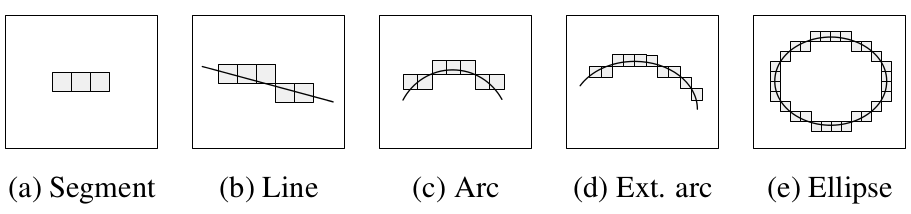
\includegraphics[width=10cm]{segs.png}}
\caption{اشکال استخراج شونده در حین تشخیص \cite{geo}}
\label{fig:segs}
\end{figure}

\newpage 

\begin{figure}[h]
\centering
\frame{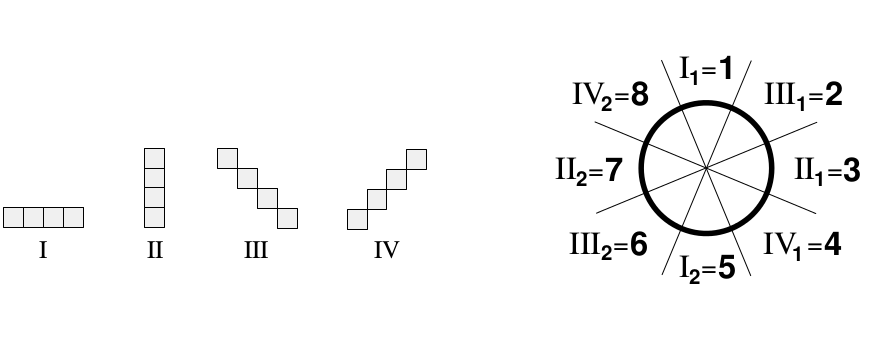
\includegraphics[width=10cm]{groups.png}}
\caption{گروه‌های خط و کمان \cite{geo}}
\label{fig:groups}
\end{figure}


\begin{figure}[h]
\centering
\frame{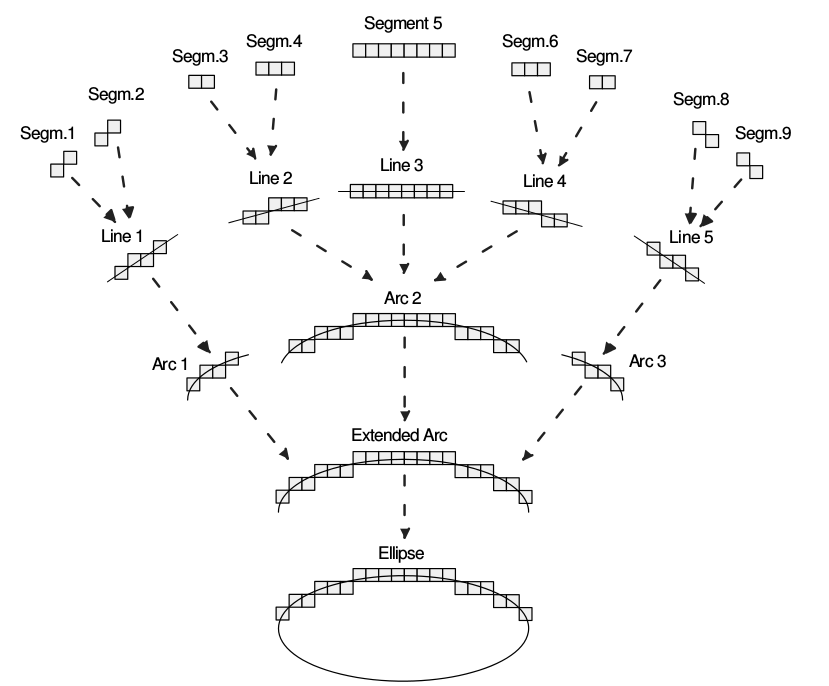
\includegraphics[width=10cm]{ell-geo.png}}
\caption{گروه‌های خط و کمان \cite{geo}}
\label{fig:ell-geo}
\end{figure}

\newpage 

\begin{figure}[h]
\centering
\frame{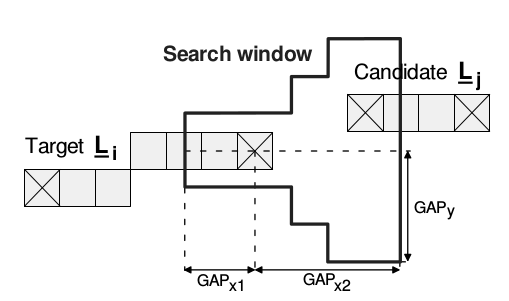
\includegraphics[width=7cm]{window.png}}
\caption{پنجره‌ی لغزان برای یافتن کمان \cite{geo}}
\label{fig:ell-geo}
\end{figure}


\begin{figure}[h]
\centering
\frame{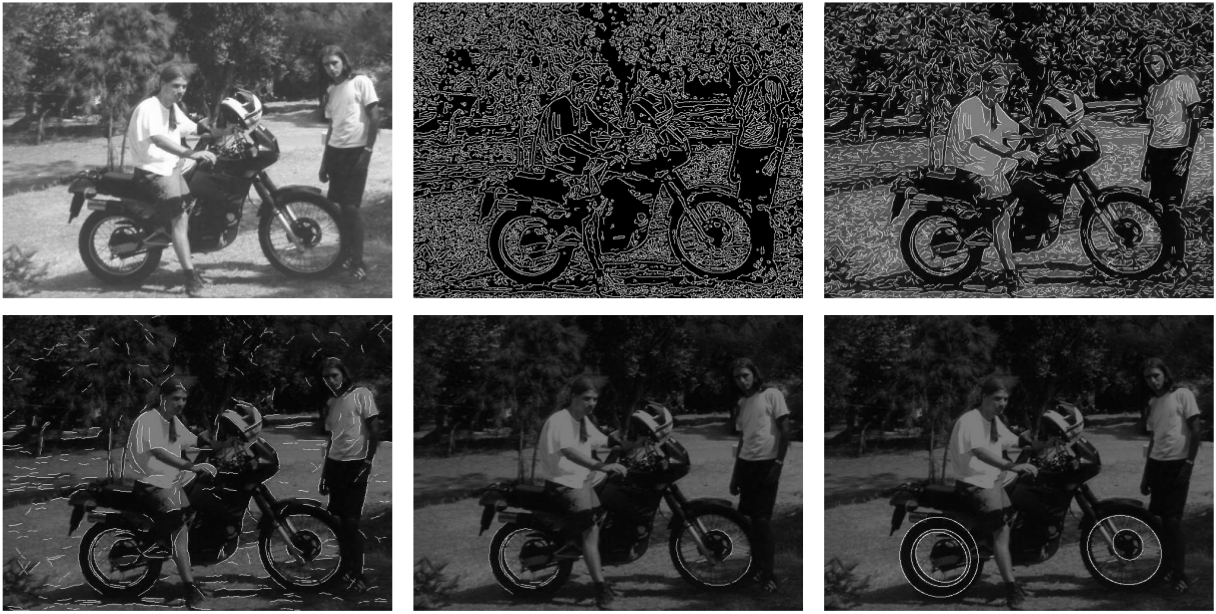
\includegraphics[width=\textwidth]{res1.png}}
\caption{نتیجه‌ی نهایی \cite{geo}}
\label{fig:res1}
\end{figure}


\newpage

%دستوری برای به حالت عادی درآمدن اندازه فونت‌ها 
\small
%ایجاد «مراجع»
\begin{thebibliography}{99}

\begin{LTRitems}

\resetlatinfont

\bibitem{Wiki}
http://en.wikipedia.org/wiki/Ellipse

\bibitem{param}
G. Song and H. Wang, “A fast and robust ellipse detection algorithm based on pseudo-random sample consensus,” in Proceedings of the 12th international conference on Computer analysis of images and patterns. Springer-Verlag, 2007, pp. 669–676.

\bibitem{diam}
D. Barwick, “Very fast best-fit circular and elliptical boundaries by chord data,” IEEE transactions on pattern analysis and machine intelligence, pp. 1147–1152, 2008.

\bibitem{survey}
Wong, C. Y., S. C. F. Lin, T. R. Ren, and N. M. Kwok. “A survey on ellipse detection methods,” In Industrial Electronics (ISIE), 2012 IEEE International Symposium on, pp. 1105-1110. IEEE, 2012.


\bibitem{fuzzy}
R. Dave, “Generalized fuzzy c-shells clustering and detection of circular and elliptical boundaries,” Pattern Recognition, vol. 25, no. 7, pp. 713–721, 1992.

\bibitem{hough}
R. Duda and P. Hart, “Use of the hough transformation to detect lines and curves in pictures,” Communications of the ACM, vol. 15, no. 1, pp. 11–15, 1972.

\bibitem{GHT}
D. Ballard, “Generalizing the hough transform to detect arbitrary shapes,” Pattern recognition, vol. 13, no. 2, pp. 111–122, 1981.

\bibitem{SLHT}
P. Nair, A. Saunders et al., “Hough transform based ellipse detection algorithm,” Pattern Recognition Letters, vol. 17, no. 7, pp. 777–784, 1996.

\bibitem{FEHT}
N. Guil and E. Zapata, “Lower order circle and ellipse hough transform,” Pattern Recognition, vol. 30, no. 10, pp. 1729–1744, 1997.

\bibitem{RHT}
R. McLaughlin, “Randomized hough transform: Improved ellipse detection with comparison1,” Pattern Recognition Letters, vol. 19, no. 3-4, pp. 299–305, 1998.

\bibitem{ellipticalHT}
C. Chien, Y. Cheng, and T. Lin, “Robust ellipse detection based on hierarchical image pyramid and hough transform,” JOSA A, vol. 28, no. 4, pp. 581–589, 2011.

\bibitem{EKF}
J. Porrill, “Fitting ellipses and predicting confidence envelopes using a bias corrected kalman filter,” Image and Vision Computing, vol. 8, no. 1, pp. 37–41, 1990.

\bibitem{RANSAC}
R. Bolles and M. Fischler, “A ransac-based approach to model fitting and its application to finding cylinders in range data,” in International Joint Conference on Artificial Intelligence, pp. 637–643, 1981.

\bibitem{GA}
P. Yin, “A new circle/ellipse detector using genetic algorithms,” Pattern Recognition Letters, vol. 20, no. 7, pp. 731-740, 1999.

\bibitem{pRANSAC}
G. Song and H. Wang, “A fast and robust ellipse detection algorithm based on pseudo-random sample consensus,” in Proceedings of the 12th international conference on Computer analysis of images and patterns. Springer-Verlag, pp. 669–676, 2007.

\bibitem{mulGA}
N. Kharma, H. Moghnieh, J. Yao, Y. Guo, A. AbuBaker, J. Laganiere, G. Rouleau, and M. Cheriet, “Automatic segmentation of cells from microscopic imagery using ellipse detection,” Image Processing, IET, vol. 1, no. 1, pp. 39–47, 2007.

\bibitem{grow}
K. Kanatani and N. Ohta, “Automatic detection of circular objects by ellipse growing,” International Journal of Image and Graphics, vol. 4, no. 1, pp. 35–50, 2004.

\bibitem{comb}
S. Tsuji and F. Matsumoto, “Detection of ellipses by a modified hough transformation,” Computers, IEEE Transactions on, vol. 100, no. 8, pp. 777–781, 1978.

\bibitem{geo}
L. Libuda, I. Grothues, and K. F. Kraiss, “Ellipse detection in digital image data using geometric features,” In Advances in Computer Graphics and Computer Vision. Springer Berlin Heidelberg, pp. 229-239, 2007. 

\bibitem{decompose}
C. Ho and L. Chen, “A fast ellipse/circle detector using geometric symmetry,” Pattern Recognition, vol. 28, no. 1, pp. 117-124, 1995.

\bibitem{FHT}
H. Li, M. A. Lavin and R. J. Le Master, “Fast Hough transform: A hierarchical approach,” CVGIP 36, pp. 139-161, 1986.

\bibitem{RHT-old}
L. Xu, E. Oja, and P. Kultanen, “A new curve detection method: randomized Hough transform (RHT),” Pattern recognition letters, vol. 11, no. 5, pp. 331-338, 1990.

\bibitem{rht-cent}
H. K. Yuen, J. Illingworth, and J. Kittler, “Detecting partially occluded ellipses using the Hough transform,” Image and Vision Computing, vol.7, no. 1, pp. 31-37, 1989.

\bibitem{PHT}
N. Kiryati, Y. Eldar, and A. M. Bruckstein, “A probabilistic Hough transform,” Pattern recognition, vol. 24, no. 4, pp. 303-316, 1991.

\bibitem{GSHT}
C. T. Ho, and L. H. Chen, “A fast ellipse/circle detector using geometric symmetry,” Pattern Recognition, vol. 28, no. 1, pp. 117-124, 1995.

\bibitem{cluster}
C. A. Basca, M. Talos, and R. Brad, “Randomized Hough transform for ellipse detection with result clustering,” In Computer as a Tool, The International Conference on, EUROCON, vol. 2, pp. 1397-1400, 2005.


\end{LTRitems}

\end{thebibliography}

\end{document} 
